\documentclass[]{usiinfbachelorproject}
\usepackage{subfigure}
\usepackage{float}
\usepackage{hyperref}
\usepackage{wrapfig}
\usepackage{xspace}

\newcommand {\stormed}[0]{StORMeD\xspace}
\newcommand {\etal}[0]{\emph{et al.\xspace}}
\author{Marco Bedulli}

\title{CSI:Cub8}
\subtitle{Augmenting Software System Representation with Corollary Information}
\versiondate{\today}

\captionsetup{labelfont={bf}}


\begin{committee}
%With more than 1 advisor an error is raised...: only 1 advisor is allowed!
\advisor[Universit\`a della Svizzera Italiana, Switzerland]{Prof. Dr.}{Michele}{Lanza}
%You can comment out  these lines if you don't have any assistant
\assistant[Universit\`a della Svizzera Italiana, Switzerland]{}{Luca}{Ponzanelli}
\assistant[Universit\`a della Svizzera Italiana, Switzerland]{Phd.}{Andrea}{Mocci}

\end{committee}

\abstract {Understanding a software system is one of the most time-consuming activities of a developer. The information that is available for a piece of code could come from the code itself or from online resources. One of the most well known  Q\&A website in which a huge amount of information is available on StackOverflow.
All this information is useful to understand the information coverage of a software system. The information not strictly related to a software system, likes forum discussions and code documentation can be useful to understand how much knowledge is available about the source code. This information comes from different sources and  there is no way to visualize in once. Collecting this data and using some visualisation method could helps the developer to spot the part of the code that require more documentation or they could give an idea about the effort require to understand the software system. Cub8 uses an augmented city metaphor as visualization method, it allow the developers to evaluate the information coverage of the system. A developer is thus able to visualize which part needs more documentation and also directly access the online information related to it.
}

\begin{document}

\maketitle

\tableofcontents 
\newpage


\listoffigures
\newpage


%%%%%%%%%%%%%%%%%%%%%%%%%
\section{Introduction} \label{introduction}

%The main purpose of this thesis is offering to the developers a way to get an impression at first glance about the information coverage of a software in an immediate and intuitively way. Cub8 can be seen as the combination of the needs to get a better understanding of the topology of the project and the needs to find all the available information related to it visualized in a easy and fast system.
%Program understanding has been estimated to be one of the most challenging task.


Developers invest great effort recovering implicit knowledge by exploring code or by interrupting teammates. This knowledge was only saved in their memory \cite{LaToza}.
According to Corbi, developers understand programs by reading documentation, reading source code, and running the program itself\cite{Corbi}. Understanding absorbs about half of the time of developers \cite{Corbi,Guimaraes}. In fact researchers showed that developers spend more time reading than writing source code \cite{Mayrhauser}.

To alleviate this problem and try to reduce the time spent by the developers to understand the code, we propose a tool that visualize, using a 3d city metaphor, the information coverage of a system and helps the developers to spot the parts of the system that need more documentation. 
The city is created using a mix of all the information available to the code, mapped to assemble the building of the city. The use of a metaphor from the physical world is the key point that makes this system particularly intuitive and effective \cite{SoftwareWorld}. This kind of visualization empowers the capacity of the viewer to transfer existing perceptual abilities through the understanding of the representation \cite{programComp}.

R. P. Gabriel \cite{Gabriel} said that "Habitability is the characteristic of source code that enables programmer, code, bug-fixer, and people coming to the code later in life to understand his construction and his intentions[...]". 
Starting from this concept, we use this idea of habitability \cite{vssac}, where this metaphor is used as a way to allow the developers to get a better understanding of a specific software system. 

As main aim, we thought to help all the developers that, coming to the system later during its development, need to be filled in quickly about all the reference and the information available on it.
The developers can navigate and interact with all the city's components, from the folder (the basement) to all the file that compose the project (building), live in Figure \ref{fig:myO}. 


\begin{figure}[h]
	\centering
	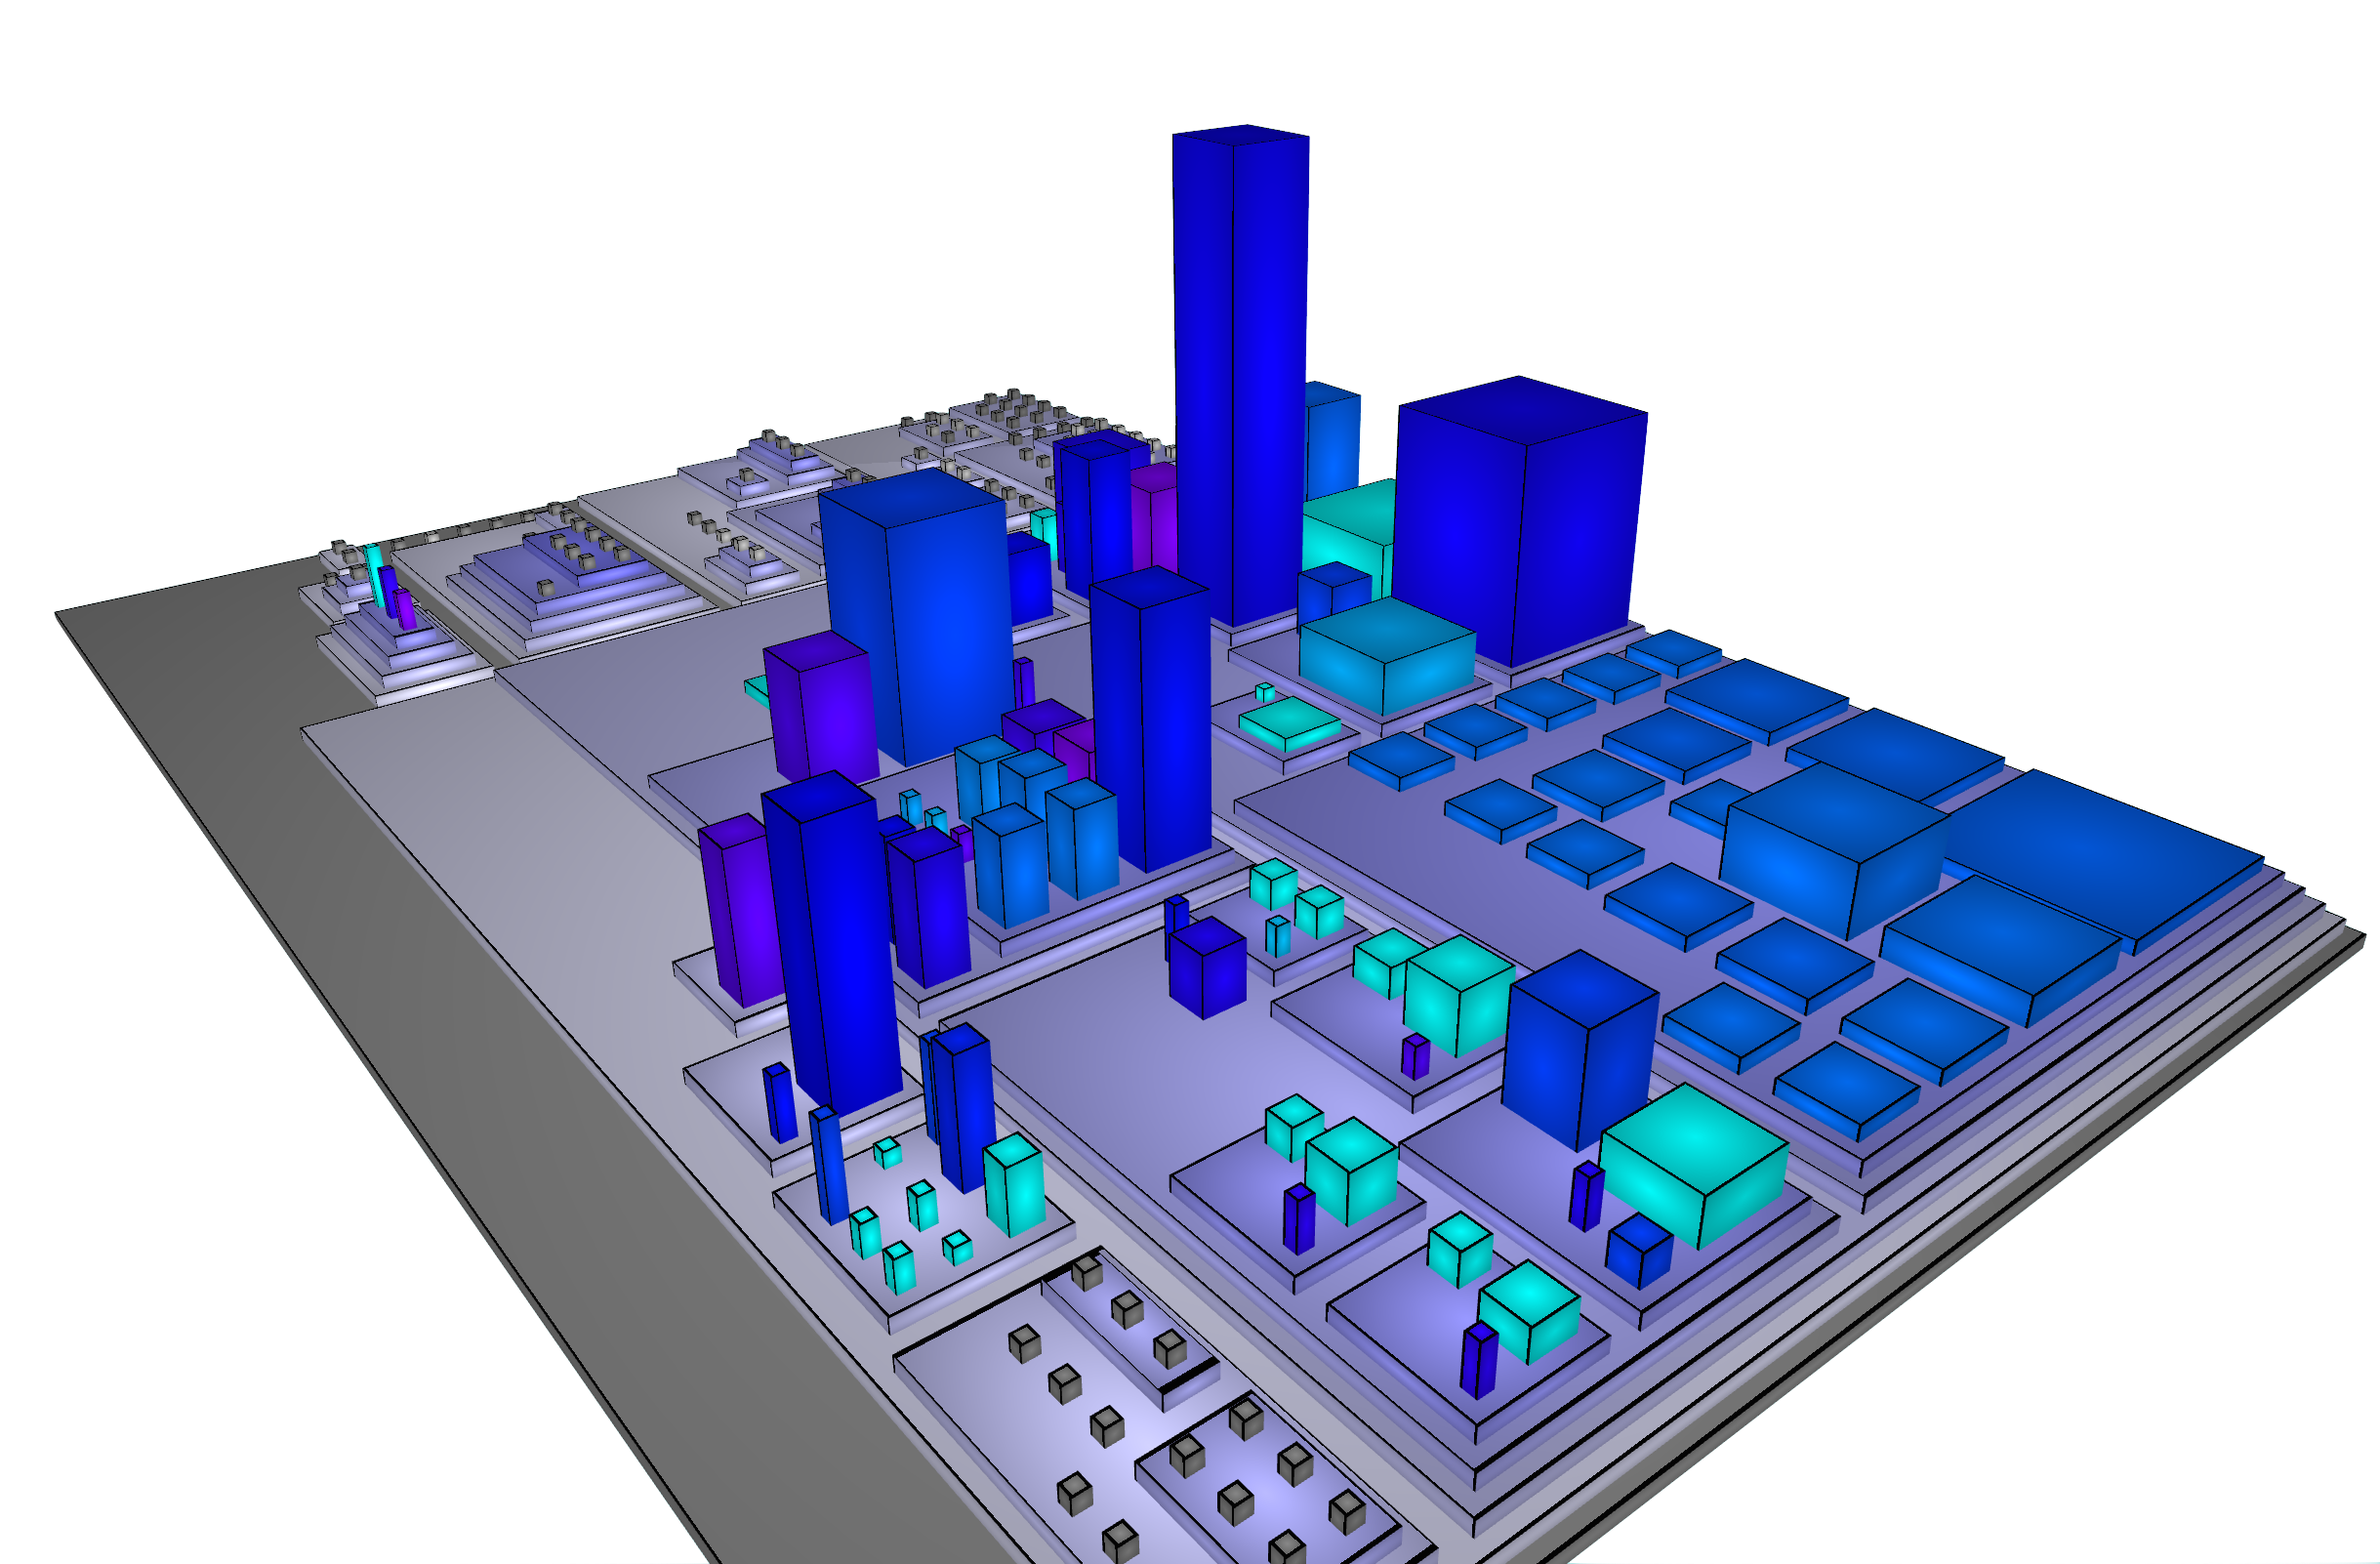
\includegraphics[width=.95\textwidth]{images/city1}
	\caption{A first example of a city\label {fig:myO}}
\end{figure}


Figure \ref{fig:myO} depicts an example of a city generated using Cube8.
Other approaches focus they intents to found code disharmony \cite{programComp} or code quality \cite{VVV} all aspect strong related to the code structure but there are no approaches that analyze the information related to a software. The developers understand programs by reading documentation, whose information is useful to reduce the effort spent by the developers to understand code \cite{Corbi}.

The information that is available for a piece of code could come from the code itself or from online resources. In both cases we refer to this data as a corollary information.
The Java doc can be used as a simple case of corollary information because it is not essential for the design purpose, but is extremely useful to understand what the code does. Usually developers do not write down knowledge in design documents \cite{LaToza}. With this tool we can spot this information issues.
The majority of the developers use Q\&A website to make  how-to questions about code issues \cite{Treude}. Stack Overflow is one example of Q\&A website, where questions are asked on a daily basis \cite{QEA}. According to the last data dump of August 2015, Stack Overflow relies on a community counting 4.5M users, who produced about 26M posts, out of which 900K questions concern the Java language. All this information is very useful through the process of code comprehension.
The goal of this thesis it to give to the developers a tool that can visualyze an entire system with all the associated corollary information. Cub8 provides a way to interact and visualize all this information coming from Stack Overflow and Java Documentations.




In Section 2 we present the related work. We describe the functionalities of Cube8 and we briefly explain how \stormed works. In Section 3, we explain the approach and the different metrics that we used. In Section 4 we show two different use cases on how Cub8 can be used and which kind of information is possible to retrieve. Finally, we present the conclusions and we discuss the future work.


\newpage


  
\section{Related Work} \label{related works}

In the past decades, researchers studied several  approaches to visualize a software system.
The basic idea is to approximate a software system to a more familiar system in which the developers are able to orient and navigate. 
There are two main metaphor for visualization methods the landscape metaphor and a city metaphor. The term landscape metaphor is not to be understood exclusively as a detailed image of reality, but rather stands for structures that are similar to those of a real landscape \cite{LS}.
The city metaphor as visualization method, used by Knight and Munro \cite{SoftwareWorld}, and Component City \cite{IDM} and later by \cite{vssac,programComp} is intended  to represent a software system as a city. The main difference between these systems is the data that they analyze.
In \cite{Evolution}  the intent is to render the structural evolution of object-oriented software systems at both a coarse-grained and a fine-grained level.
\textit{Software word} \cite{SoftwareWorld} is a system in which the buildings represents the functions, the size of a building represent the number of lines of code and the color the modifier of the function.

Wettel and Lanza \cite{programComp} propose a city metaphor in which there is a fixed number  of building types such as skyscraper, office building, apartment block,mansion, and house. They propose two mappings: boxplot-based mapping and threshold-based mapping. Also, they use a box-packing algorithm to visualize the city. The city metaphor consist into classes represented as a building located in city districts which in turn represent packages. The goal of the visualization is to show the structure of a software.  \cite{vssac}  propose a 3d environment in which the software system is represented as a city, whit different class of buildings. It also implements a way to navigate and interact with the system. It is possible to select any artifacts and interact with them, spawning complementary views(i.e., a tagging system and a query system).
Tymchuk \etal \cite{VVV} propose an approach to augment code review by integrating software quality evaluation, and more general design assessment, not only as a first class citizen, but as the core concern of code review.
In Cub8 we have  get some of this ideas: the navigation and the interaction through the system and the boxing building methodology to generate the city but we also delegate to the user the decision of  the different metrics to assign to the dimensions of a building.  
The corollary information that we are using to give to the developers a more complete idea about the information available is taken from Stack Overflow. We use the \stormed dataset, it consists of a set of JSON files that contain an H-AST of each discussion. It implements an island-parsing algorithm \cite{stormed}. There are also other approaches that used Stack Overflow as a  way to retrieve data.

SISE \cite{SISE}  use machine learning based approach where the features are the sentences themselves, their formatting, their question, their answer,  their authors ,the part-of-speech tags and the similarity of a sentence to the corresponding API.
Arwan \etal \cite{7231439}  proposes a mechanism for finding code on Stack Overflow uses Latent Dirichlet Allocation (LDA) using concept location in the preprocessing stage. 
 


\newpage
\section{Approach} \label{approach}

Cub8 allows the developers to apply different metrics on a city and  mix different views together to get a global idea about the system coverage. In this chapter we are going to exploit and analyze what these metrics does and which kind of information is possible to retrieve. 
We concentrate our studies on Java based system. Java is a well known Object oriented language and therefore we refer to classes, interfaces, methods and fields as the main part of project.
We also use some notation for identify the different metrics: 
\begin{itemize}
\item NOM: Number of Methods, represent the number of method declarations contained in a file 
\item NOF: Number of Fields, represent the number of fields contained in a file. 
\item NOJ: Number of Java Documentation, count how many method declaration are commented; its absolute value represent the number of method documented, its percentage represent the number of method  documented over the total amount of the methods of the file.
\item NOD: Number of Forum Discussion, count how many method call and import are discussed; its absolute value represent the number of method call and import discussed, its percentage represent the number of method call and import discussed over the total amount of the possible method call and import. We do not count local package and methods that are declare in the project.
\end{itemize} 

\subsection{Information strictly related to the code}
The code related information are used to give to the developers a better understanding about the locality of the code. To demonstrate this concept we compare two different cities computed on the same code. The system  consists of only two classes. ClassA has 4 methods and ClassB has 4 methods plus 4 other fields. The main goal of this example is to find which class needs more documentation. 

Figures \ref{fig:strictly:a} and \ref{fig:strictly:b} show the mapping; the color schema goes from light blue to purple.
Purple mean the maximum and light blue the minimum amount of data either  in percentage or in an absolute value.
In \ref{fig:strictly:a} the color represent the NOJ and in \ref{fig:strictly:b} the NOM.
In Figure \ref{fig:strictly:a}, we can notice that the big building on the left has adequate documentation, instead, the right one has no documentation. By looking at the mapping and the class description ClassA is our target, in fact it is thin and tall this means that it has the NOM >> NOF.
In Figure \ref{fig:strictly:b} instead we represent more corollary information at the same time using different axes. The city becomes unusable because it is indistinguishable which is the ClassA and which is the ClassB since the only difference is on the number of fields. Figure \ref{fig:strictly:b} the developers can make some general observation about the relationship between java documentation and discussions.
Later in this section, we are going to analyze in more detail the color metrics system and the purpose of the other adopted metrics.

 
 
 
 




\begin{figure}[H]
	\centering
	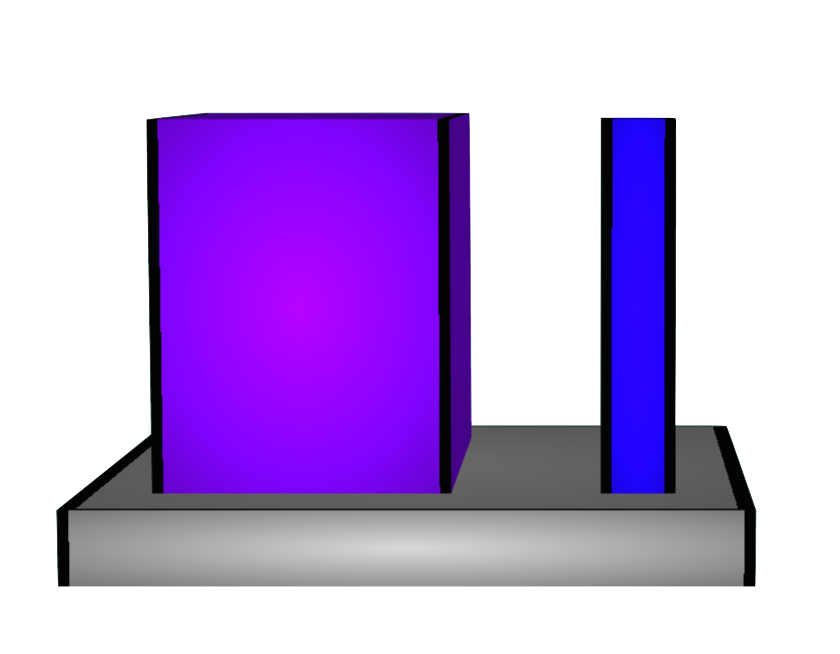
\includegraphics[width=.45\textwidth]{images/correctC}
	\caption[Methods and Fields]{Mapping as Width: number of methods, height: number of fields, colour: javaDoc\label {fig:strictly:a}}
\end{figure}



\begin{figure}[H]
	\centering
	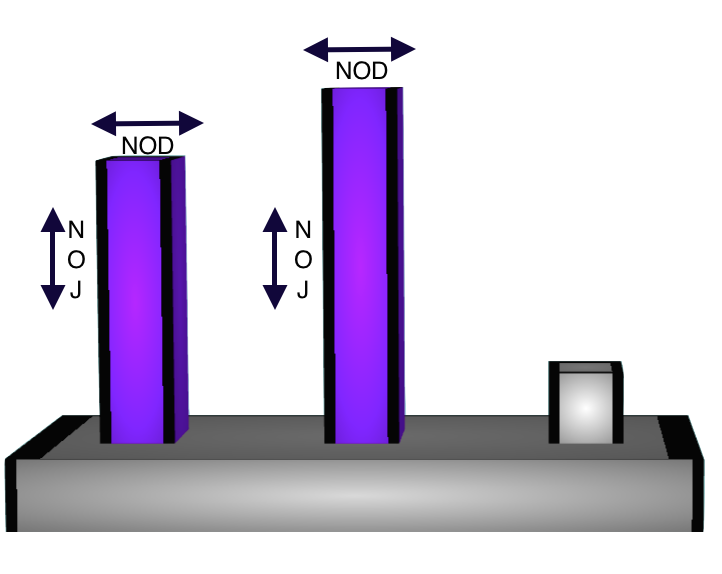
\includegraphics[width=.45\textwidth]{images/wrongC}
	\caption[Discussions and Java documentations]{Mapping as width: number of discussions , height: number of Java documentations, color: number of methods \label {fig:strictly:b}}
\end{figure}




\subsubsection{Classes and interfaces}

Classes and Interface are the only two possible code containers in Java. Cub8 allows the developers to analyse their distribution and highlight possible bad design choics.
Note that as Oracle \cite{oracle} says: "Each Java source file contains a single public class or interface. When private classes and interfaces are associated with a public class, the developers can put them in the same source file as the public class", the direct consequence that arises is that we could have more classes in a single source file and therefore it is also legal to have buildings with different size on the resulted city.

When there are to many classes in the same file, an important information that can be retrieve from this visualization is the average level of coupling in the code. In a file with a huge amount of classes; there could be a high degree of coupling, could it will be harder to maintain it. We will discuss an example of this representation method during the analysis of TomCat in Section 4. 





\begin{figure}[H]
	\centering
	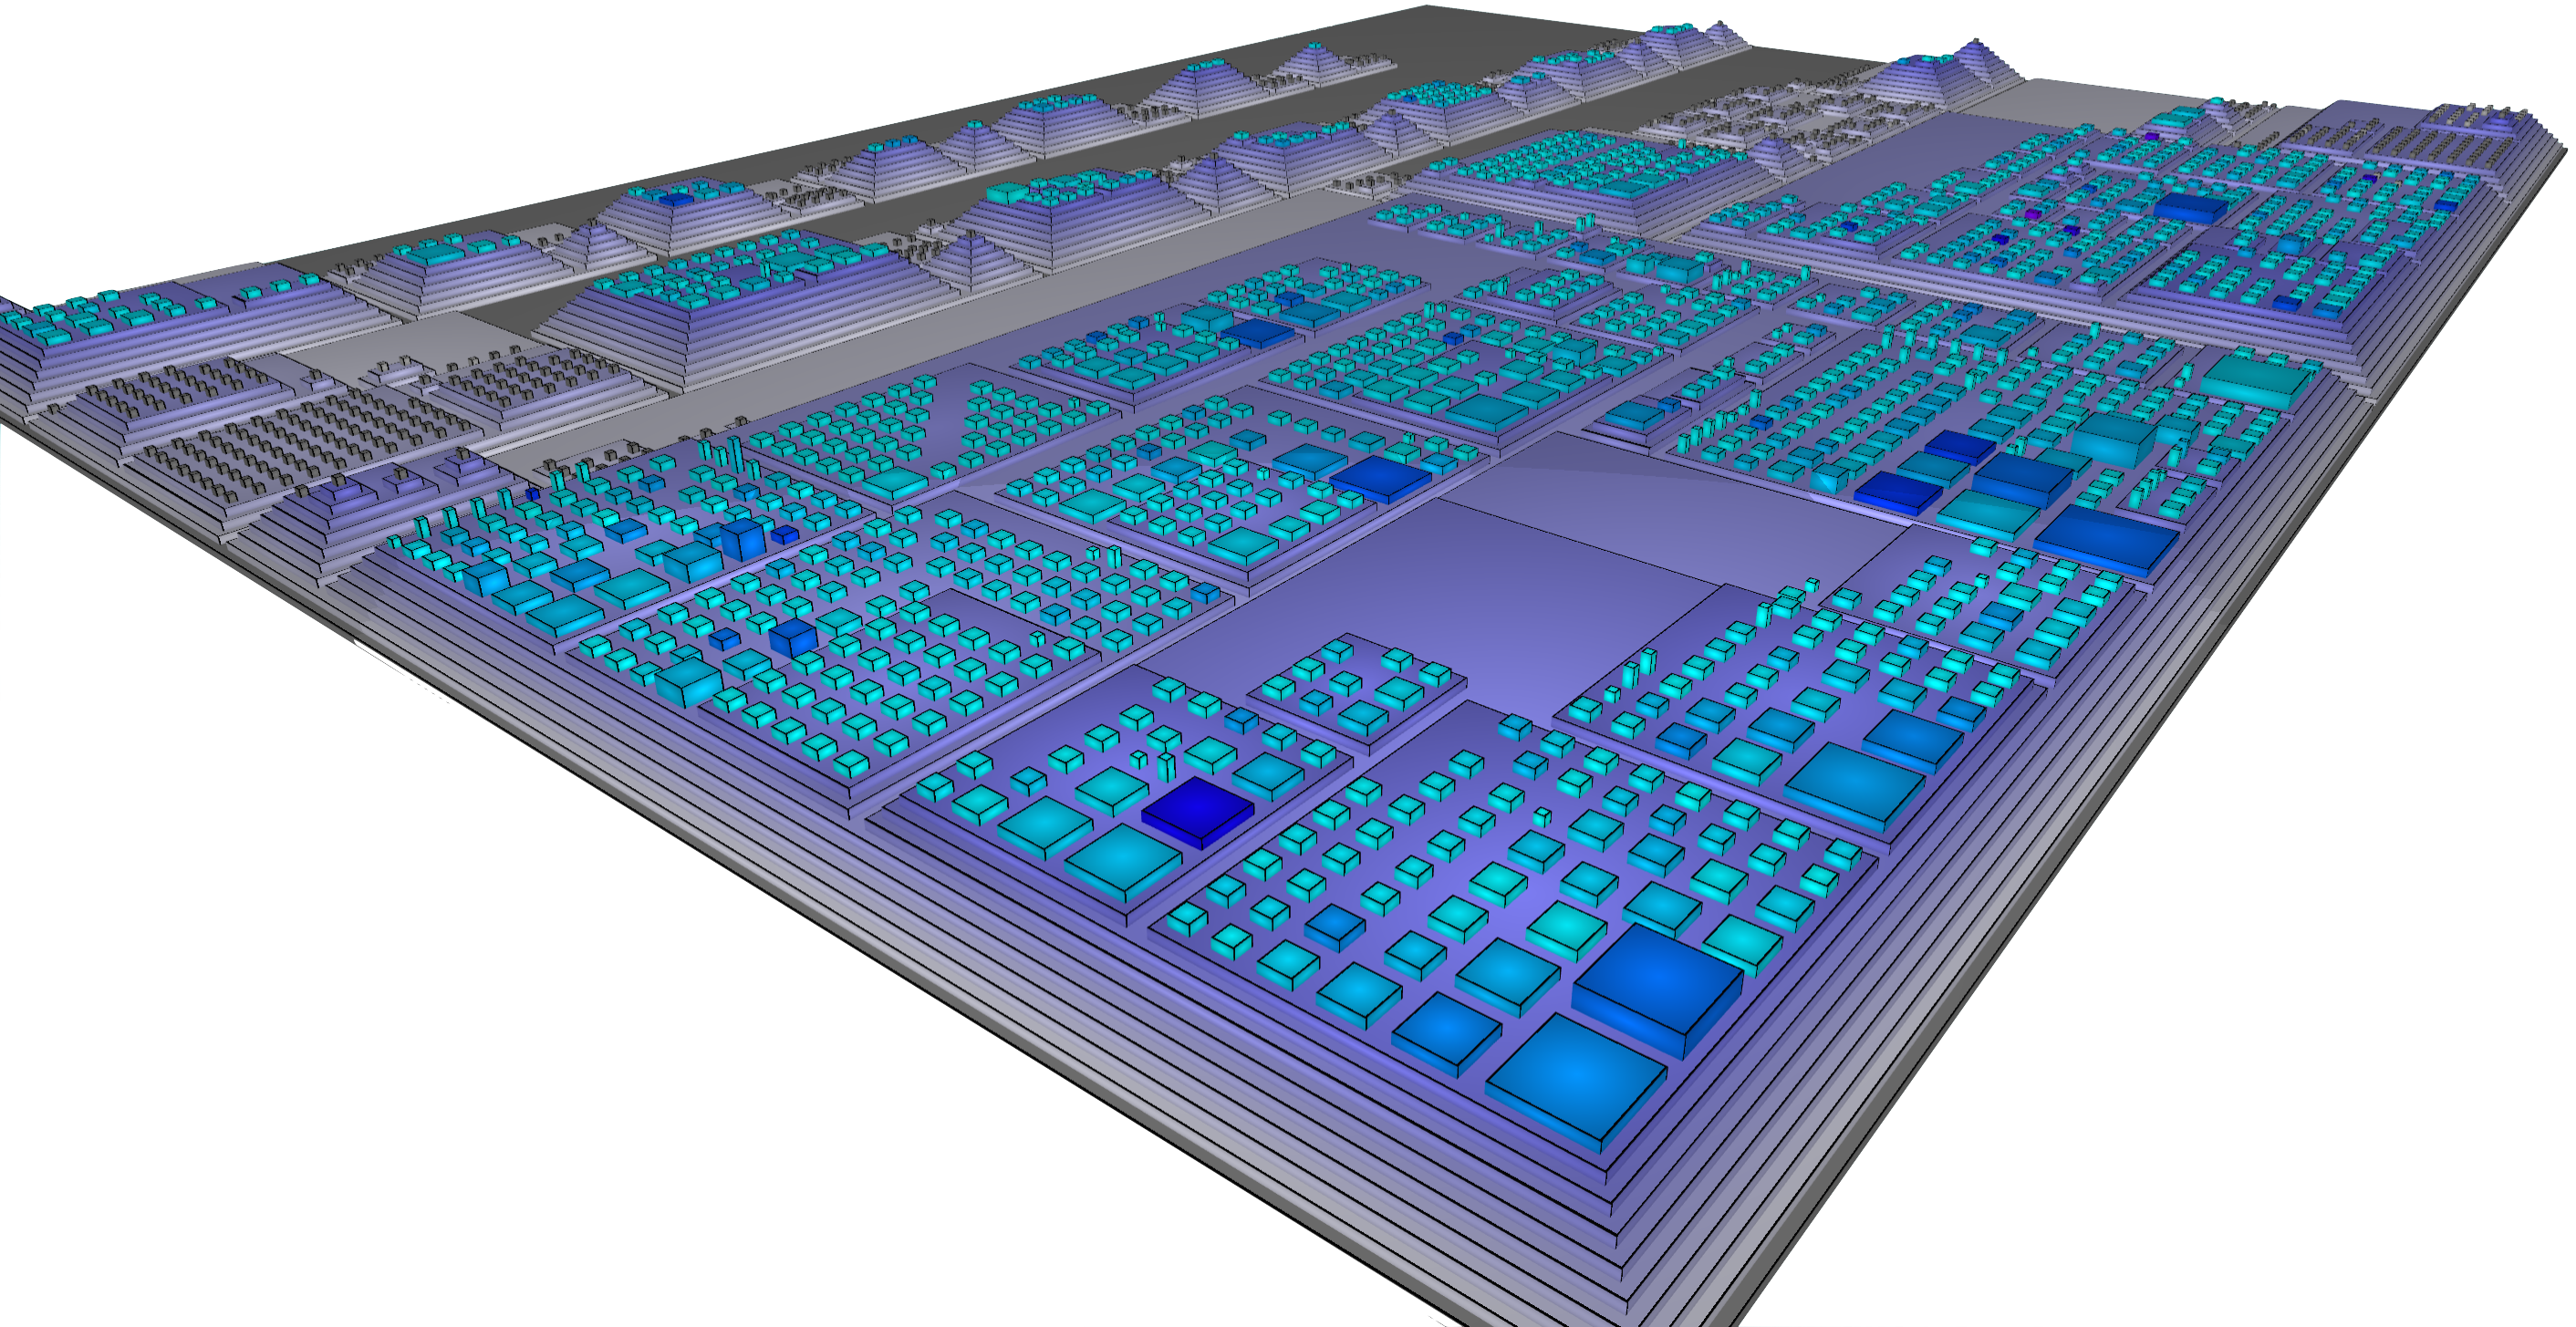
\includegraphics[width=.95\textwidth]{images/ClassesAndInterfaces}
	\caption[Classes and Interfaces Mapping]{Mapping as Width:Number of Classed, Height: Number of interfaces \label{fig:classInterface}}
\end{figure}


Figure \ref{fig:classInterface}, shows an example where we analyze this two concepts in a big project. There are a few classes that need some check to make sure that this design principle is respected. We use the width to show that it is possible to change metrics respect to what we are going to look at. Recall the concept of habitability \cite{programComp} we could also maintain the building size as NOM and NOF and changing the color depending of the number of classes. In this way we can still have a idea about the class distributions and keep the structure unchanged. 


\subsubsection{Identity harmony	}\label{sec:idHarmony}

Design disharmonies are formalised design shortcomings to detonate pieces of system that exhibit design problem \cite{Disharmony}. 
There are three different type of harmony:
\begin{itemize}
\item Identity harmony: every entity in the system must justify its existences.
\item Collaboration Harmony:  the entity collaborate from each other to perform operations.
\item Classification Harmony: The entity could inherit from other entity. 
\end{itemize} 
With our tool we can only identify some of the identity harmony. We do not visualize any of the relationship between classes(inheritance) or method collaborations.
The three identity harmony that we are able to visualize are
\begin{itemize}
\item{God Class}: it is a class that does too much. In our representation appear like a big box.
\item{Brain Class}: it is a class that accumulate an excessive amount of intelligence,usually has a lot of methods: it is look like an antenna
\item{Data Class}: it is a class that hold a lot of data and does not perform any operation:it appear to a be a big and thin box.

\end{itemize} 
\begin{figure}[h]
	\centering
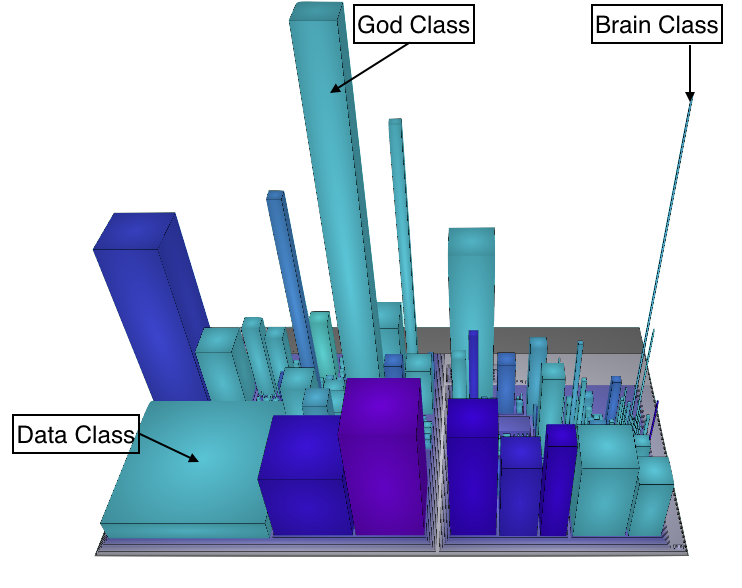
\includegraphics[width=8cm]{images/disharmony}

\caption{Identity harmony\label {fig:harmony}}
\end{figure}

Figure \ref{fig:harmony} is an example of this 3 kind of disharmony and how they should look like in the city representation.




\subsubsection{Methods  and fields}



Methods and fields are the main elements that compose a class. We are using this two measure to draft the size of the buildings. The reason why we choose this pair is that they give the correct granularity to have a better perception of the system; Wattel and Lanza  \cite{Disharmony,vssac} use the same mapping. Since we are interested in the visualization of the information coverage that is computed respect to  methods. 

Using this metrics we are able to  identify a potential disharmony as describe in the preview sections.
Figure \ref{fig:harmony}  shows an example of each possible disharmonies.
 


    
\newpage
\subsection{Information not strictly related to the code}
The information not strictly related to the code is the focus of this thesis. This knowledge is essential to get an idea about the complexity of understanding a software system and where more effort must be put. At the same time, this visualization could be used by the developers to monitor which part of their code require more documentation.


\subsubsection{Java documentation}
Collect and visualize the java documentation is the first step of the process to collect the coverage information because it is integrated with the code and it does not require any particular computations. It covers an important role in the process of understanding the functionality of a given code since is written directly by the developers and should be used in each method, field and class definitions.

This views allows the developers to spot the pieces of the system that require more documentation. We are collect only the documentation related to the methods. We choose this level of granularity because it gives a good level of details. It is impossible to have code documentation per line and is also not much useful  class documentation to understand its details. 
We usually map the java documentation using the colours. In this way we give to the developers a fast way to understand all the data information. 


\begin{figure}[H]
	\centering
	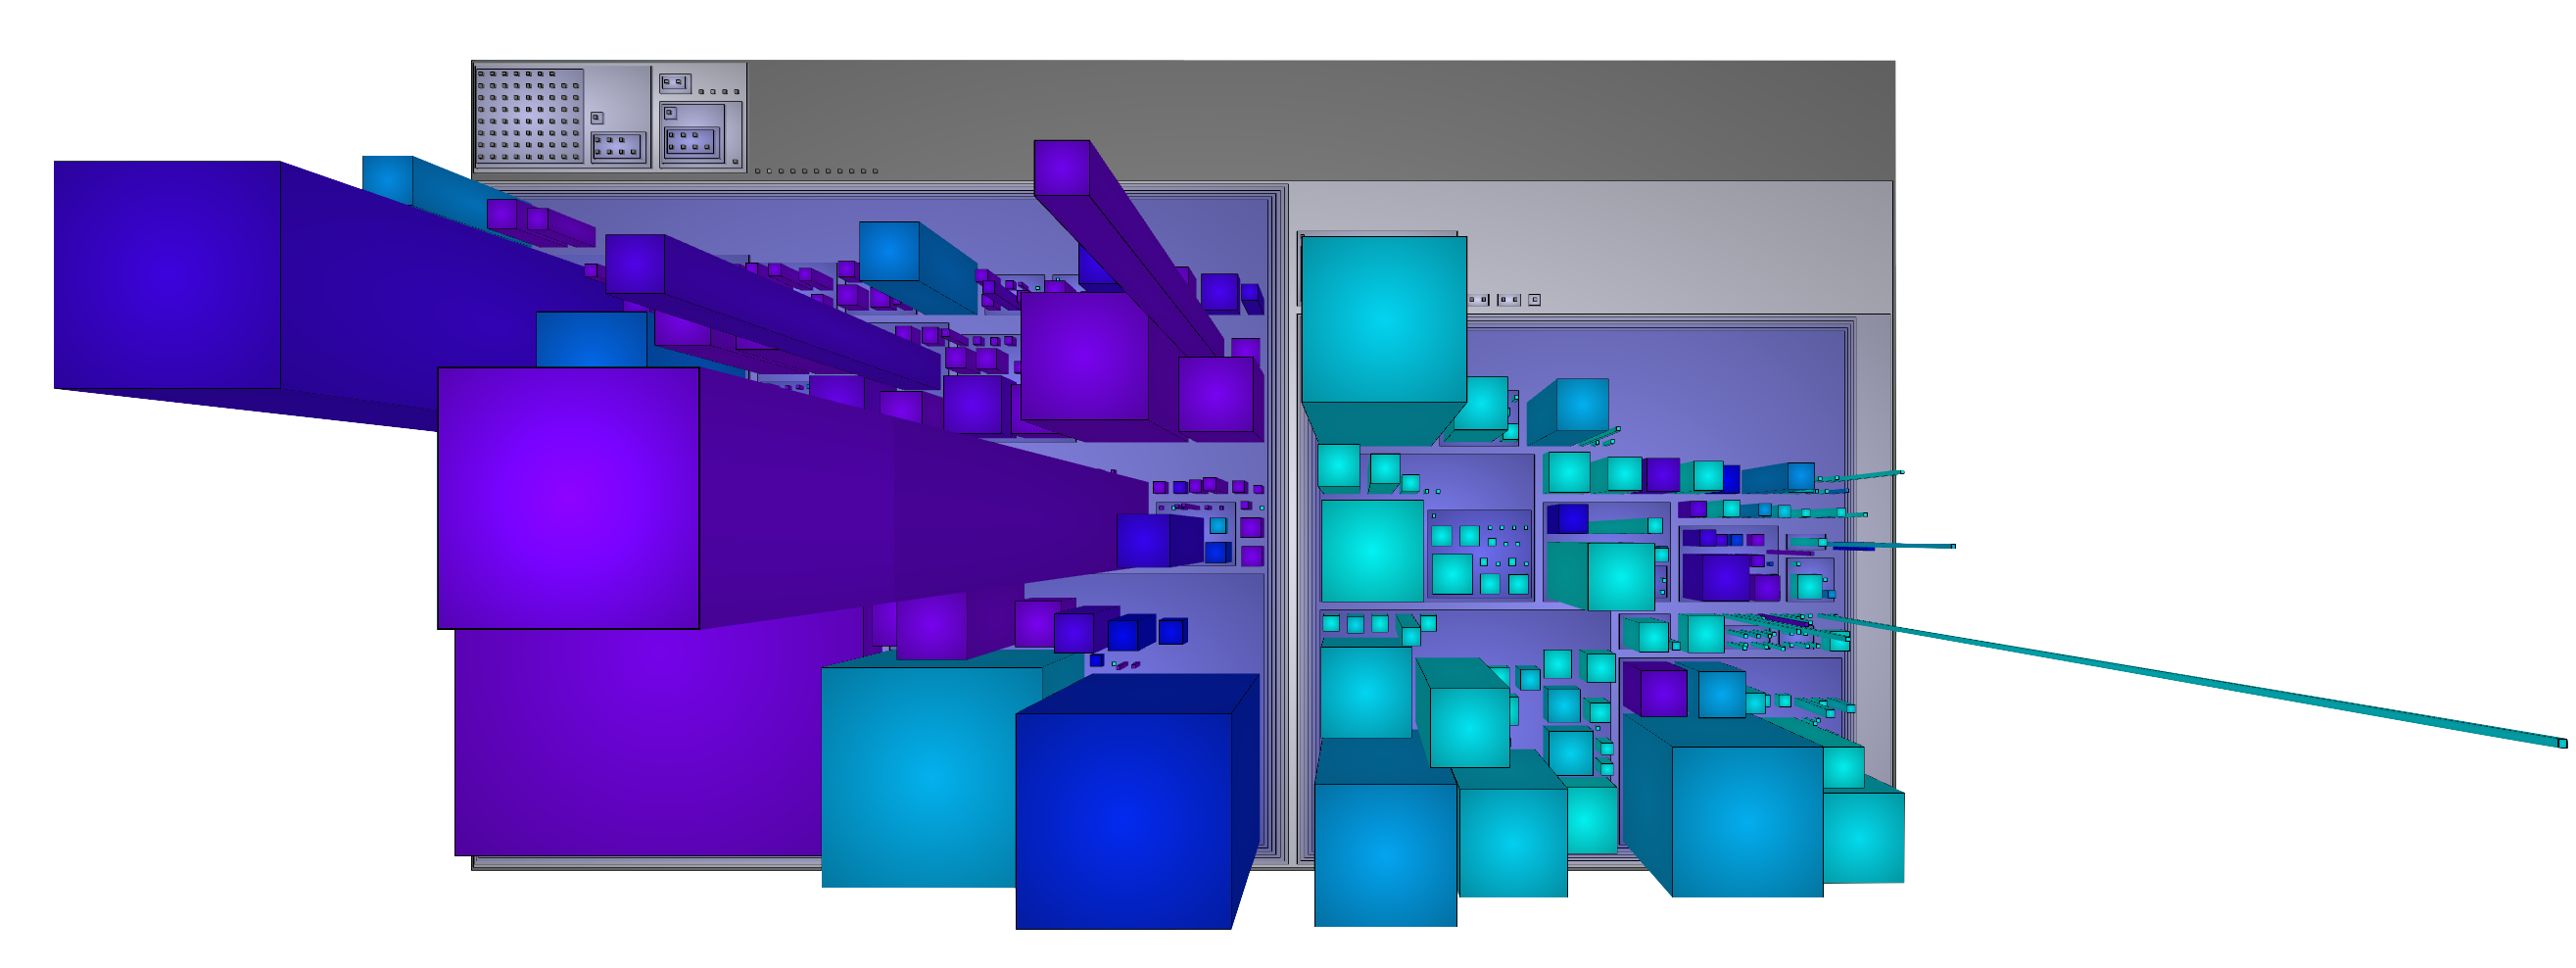
\includegraphics[width=1\textwidth]{images/javaDoc}
	
	\caption[Java Documentation Mapping]{Mapping as Width:N of Fields, height: Number of Method,Colour: Percentage of documented methods\label{fig:javaDoc}}

\end{figure}

Figure \ref{fig:javaDoc} is an example of a city in which the colour represent the percentage of documented methods of the \textit{apache common-lang}\footnote{https://commons.apache.org/proper/commons-lang/} library. It is very interesting to see that half of the project has a documentation coverage around  80\%, while the other half documentation is very limited. In reality, this is a common case as a lot of projects do not report an adequate documentation in the tests.

To help developers to fully understand the documentation coverage, we provide a  package base colouring system, where the colour of each package is the average of its child components. 
Figure \ref{fig:OnlyPackage} depicts  the same project showed in Figure \ref{fig:javaDoc}. It is more clear to see the global characteristics of the project (at package level) and it appears clear that the test are less documented than the core.

\begin{figure}[H]
	\centering
	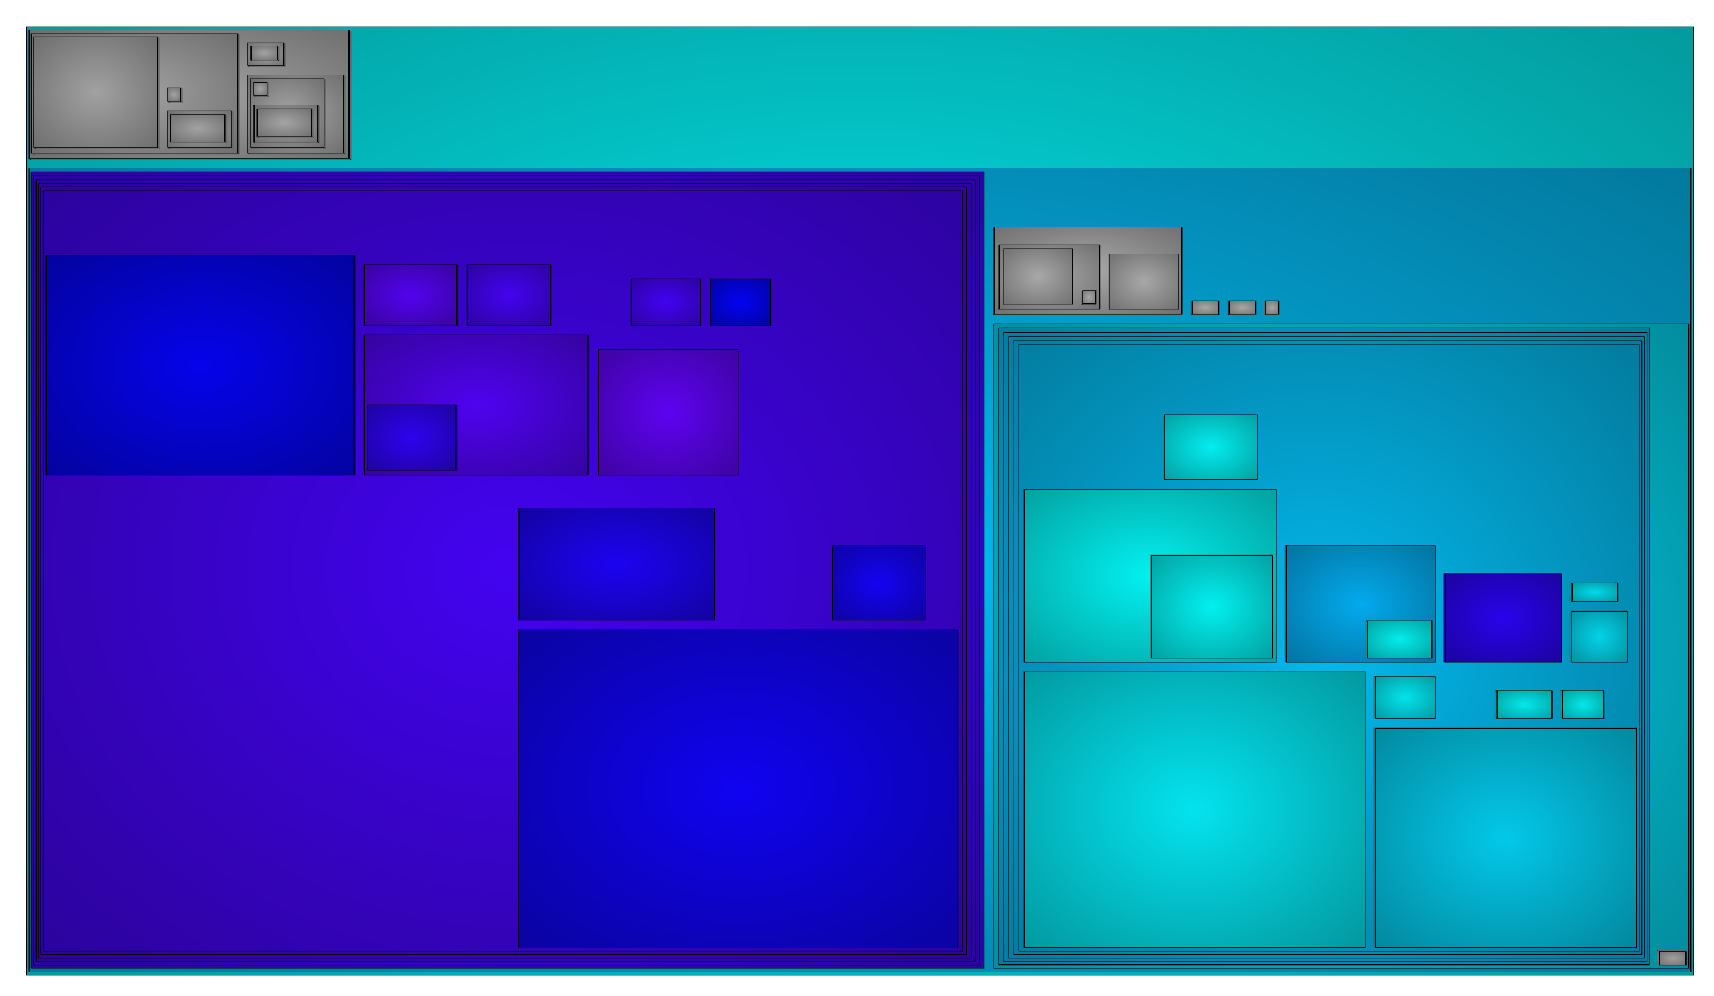
\includegraphics[width=0.5\textwidth]{images/javaDocOnlyPackage}
	
	\caption[Java Documentation Mapping Only Package]{Mapping as Width:N of Fields, height: Number of Method,Colour: Percentage of documented methods\label{fig:OnlyPackage}}
\end{figure}


\subsubsection{Stack Overflow  Discussion}

Stack Overflow\footnote{http://stackoverflow.com/} is one of the most popular Q\&A website for developers. It contains a lot of code snippets and text related to the code. What we try to do using this visualization method is to show to the user all the available discussions related to each method call. The granularity is different respect to the java doc metric. That allows understanding the complexity to read and understand the methods code not what the method itself does. We get the dataset updated in august 2015.
In this stage, we have all the repository code and all the discussions information (methods call and imports) from the \stormed  Dataset\footnote{http://stormed.inf.usi.ch/}. 
\stormed contains  the code snippet and the code reference in text of  each discussion, and provides tools to extract the method calls and the import declarations from the dataset. The  majority of the snippet are incomplete so we do not have the type of each call. Also the imports are not used in all snippets \cite{stormed}. To match the method calls found on the discussions to the method calls found in the source code we simply match the names and the number of arguments. This simplification implies some false positives. The imports are still matched using the package name.

By double-clicking over each building it is possible to get a list of the discussions found.
Figure \ref{fig:disc} is an example of the discussion found in respect to a building. The color represents the number of discussions in an absolute way. There are two classes that have more discussions that the others. Classes that have more field are colored in light blue.


\begin{figure}[H]
	\centering
	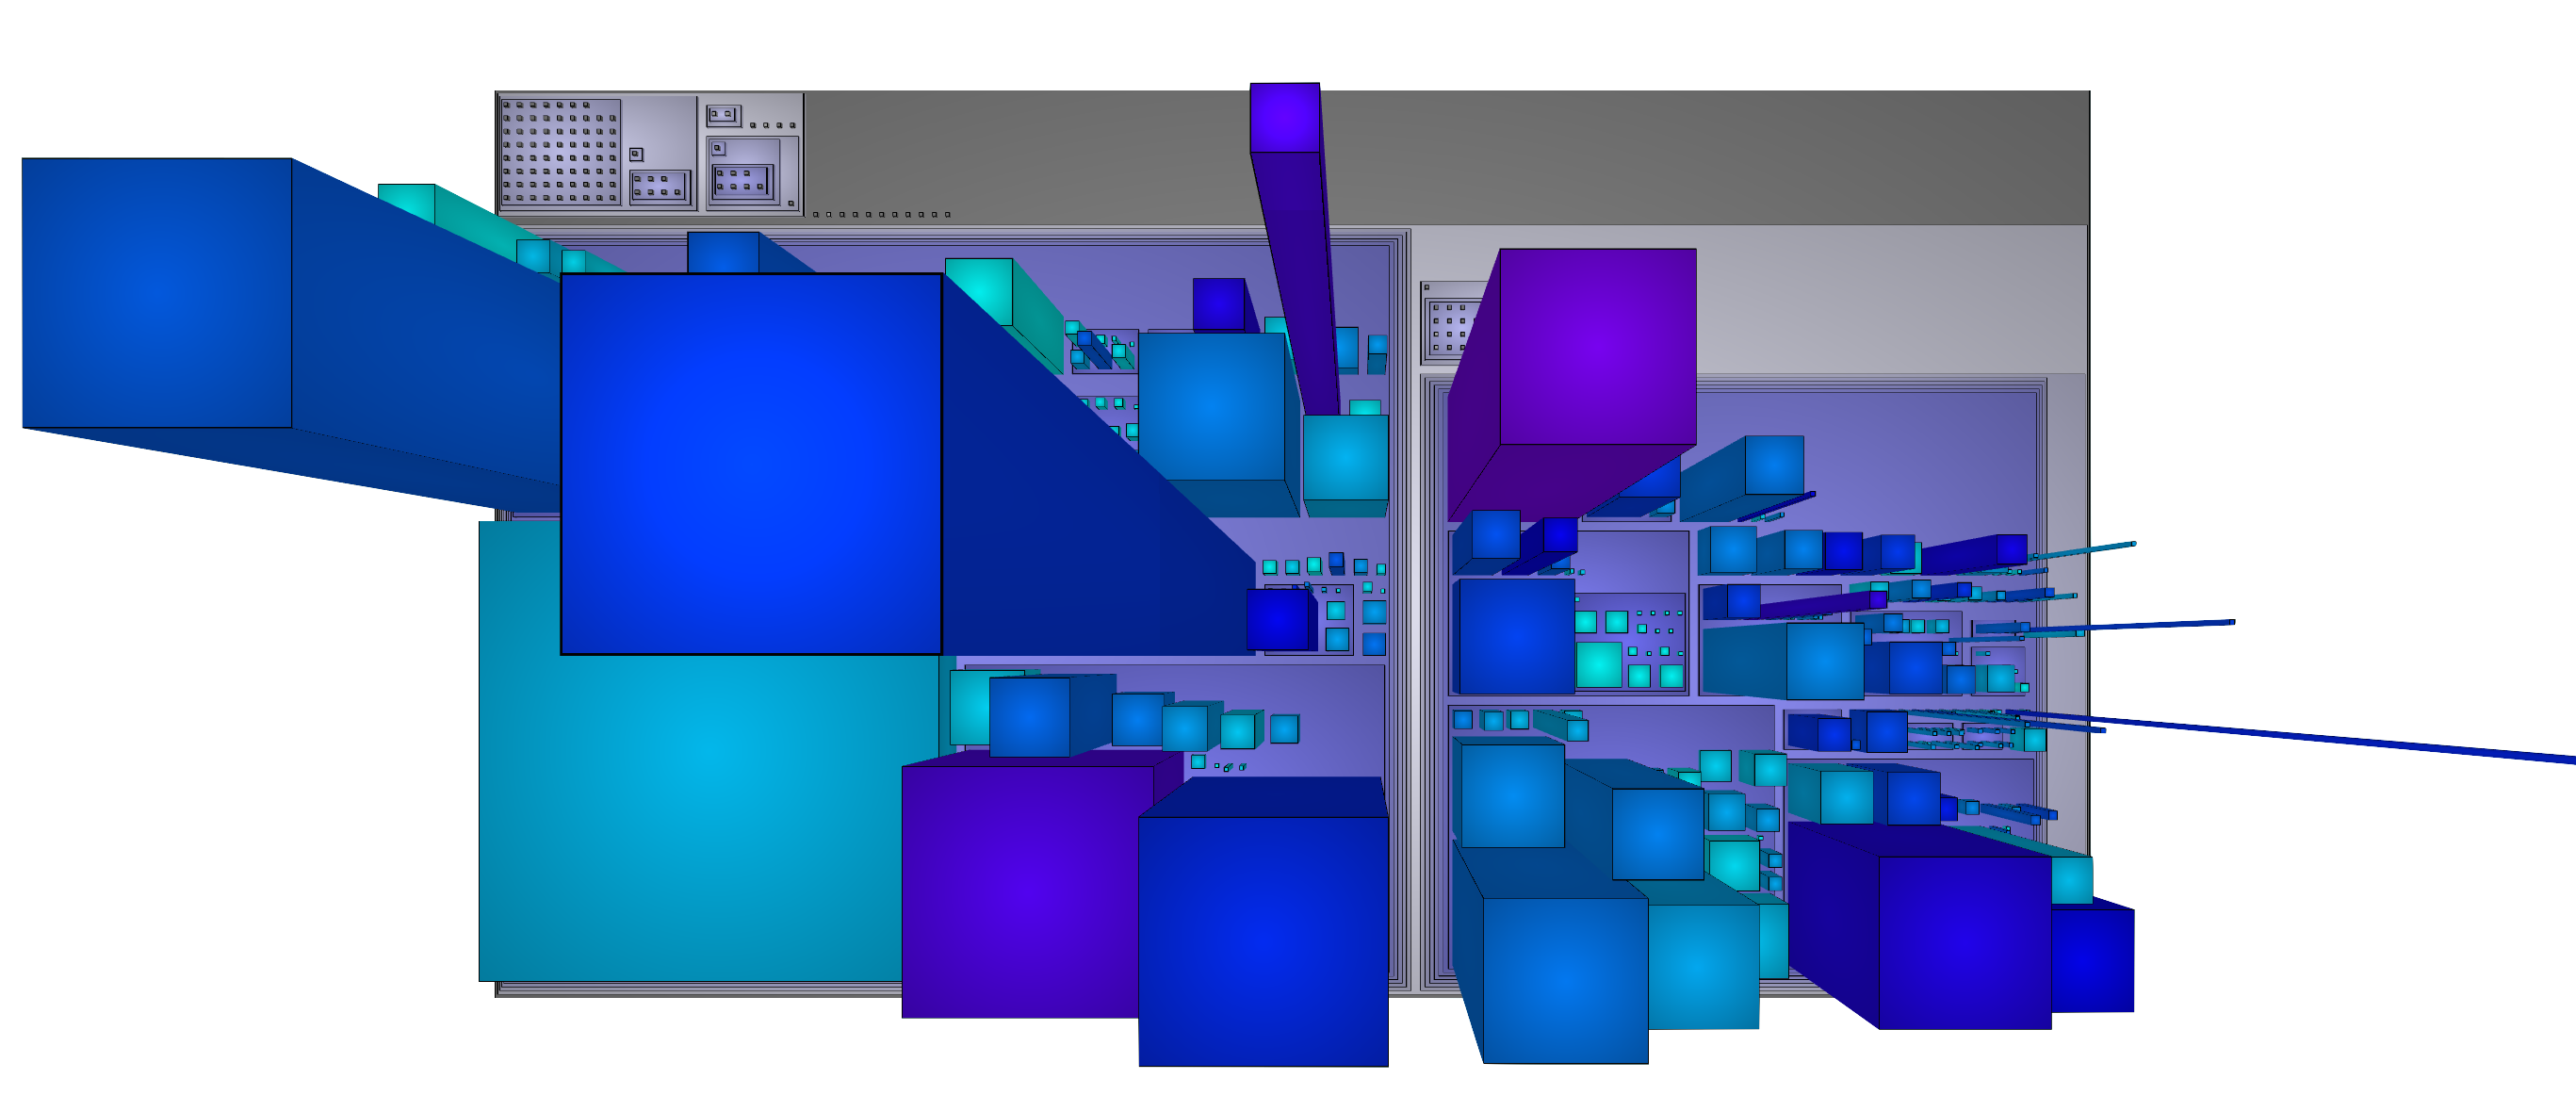
\includegraphics[width=0.8\textwidth]{images/discAbsLang}
	
	\caption[Discussion Mapping]{Mapping as Width:N of Fields, height: Number of Method,Colour: Absolute number of discussions\label{fig:disc}}

\end{figure}




Figure \ref{fig:list} shows an example of list of links for each method call or import declaration.


 \begin{figure}[H]
	\centering
	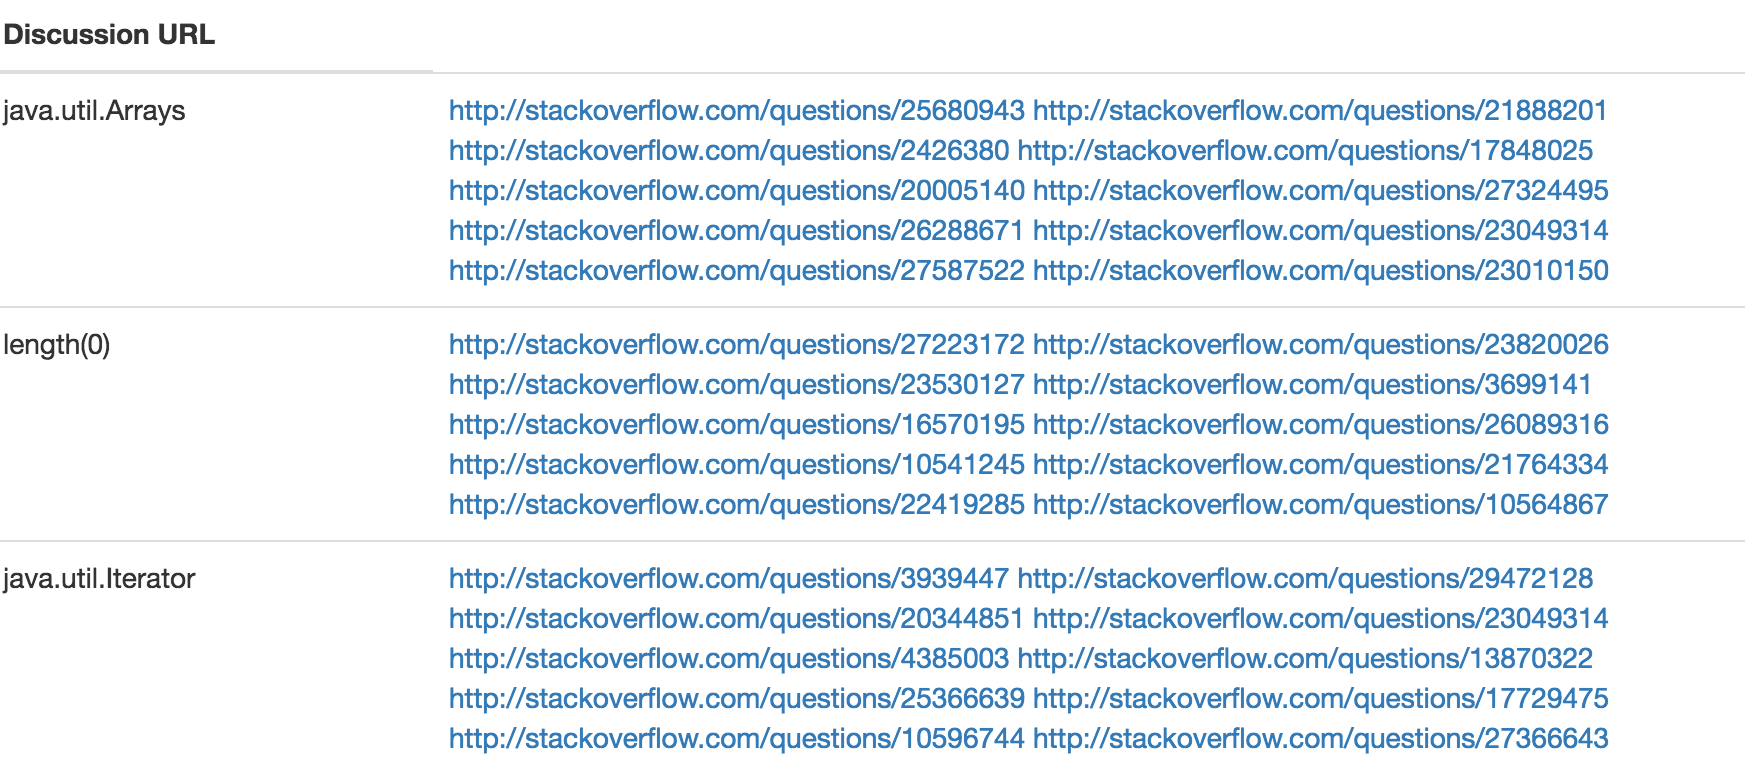
\includegraphics[width=1\textwidth]{images/listOfDiscussions}
	\caption[List Of Discussions]{List Of Discussions \label{fig:list}}
 \end{figure}


\subsection{Merge code related information with corollary information}
The code related information helps to identify the different components of the city and also it helps to find design problems over the system. The corollary information instead, gives an idea about the information coverage. How can we mix this information together to get a global overview of the entire system? In Figure \ref{fig:disc}, we use the information related to the code to give the dimension of the building, and we use the color to represent the information coverage. In this way, we improve the concept of locality since a developers should remember a file not for the number of documented methods but for his structure.

\subsubsection{Percentage and absolute number of information}

The information could be represented  as an absolute or a percentage value. In the former way, we count the number of information available and it is possible to see which file contains more information. The latter, instead, it is computed over the total amount of information that could be found. This metric is useful to spot which files have more data. A special case is the forum discussion metrics: we decide to give 0\%  were we can not find anything related to the code.
An example is the number of java doc. If we use the absolute value the color represents the number of the methods documented; otherwise, by using the percentage value, the color represent the methods documented over the total amount of the methods.


\subsubsection{Using java doc and discussions together}

To get a better understanding about the information coverage we have to join the java documentation and the information related to code. We obtain an average of both since they correspond to two difference level of granularity. The java documentation refers to a method and the discussion refers to either import or method calls. We can show the result in both ways: percentage and absolute.
In the former case, the developers can get a better understanding about the percentage of the information available. This is useful to guess the effort require to understand the system. The latter, instead, is used to see where there is more concentration of information and where is not. It could be useful to identify  bad documented packages.

  


\subsection{Colors}
The colors are used to show other metrics. They spread from light blue to purple and are very useful to give to the developers a quick impression about the system. In the next section colors are used to map corollary information and to identify some code disharmony.


\subsubsection{Corollary information colour meaning}
The color used to compute the corollary information it is computed as absolute or percentage. In the former case, the purplish building represents the file that has more information coverage; the light blue highlight the file which has less coverage. In the latter case, we see the percentage over the methods. This give a local view about the percentage coverage respect to a file.  Colors depend only on a file, not on the whole project like in absolute view.

An example is the discussion coverage. Using the percentage distribution, we get all the full discussed file in purple, independently from the number of method calls. Otherwise, using the absolute distribution we have the file with a higher number of discussions in purple.


 
\begin{figure}[h]
\centering
\subfigure[Color HSV]{
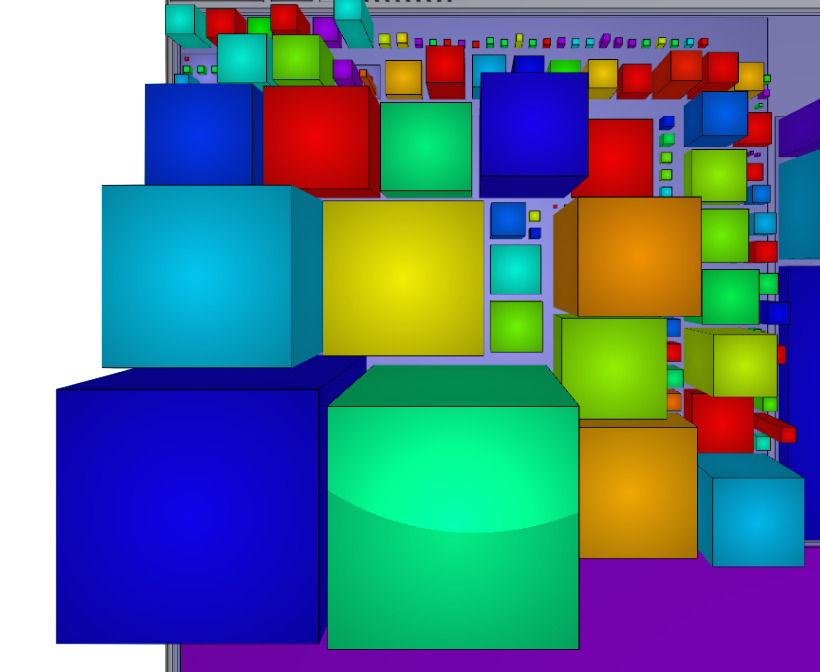
\includegraphics[width=.45\textwidth,height=4cm,keepaspectratio]{images/color}
\label{fig:color:a}
}
\hspace*{\fill}
\subfigure[Range of Colors ]{
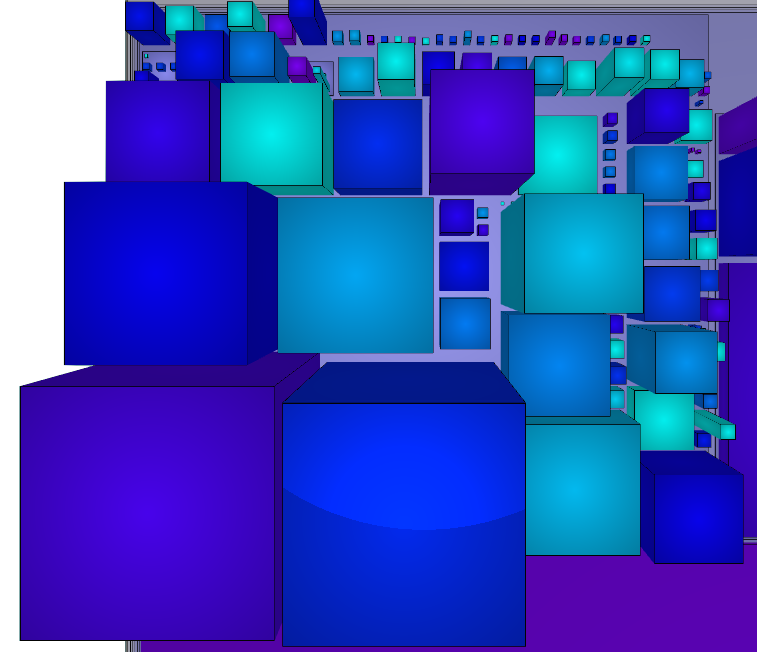
\includegraphics[width=.45\textwidth,height=4cm,keepaspectratio]{images/colorNormal}
\label{fig:color:b}
}

\caption{Colors model}
\label{fig:color}
\end{figure}

We use a subrange of the HSV color model, as shown in Figure \ref{fig:color:b}.
Figure \ref{fig:color:a}, instead, is an example where we use the whole HSV color model. The color goes from red to purple pass thought yellow, green and blue. 
By comparing Figure \ref{fig:color:a} and Figure \ref{fig:color:b} we note that the whole HSV color model adds more noise to the representation making the city hard to be understand.\begin{figure}[h]
\centering
\subfigure[Absolute]{
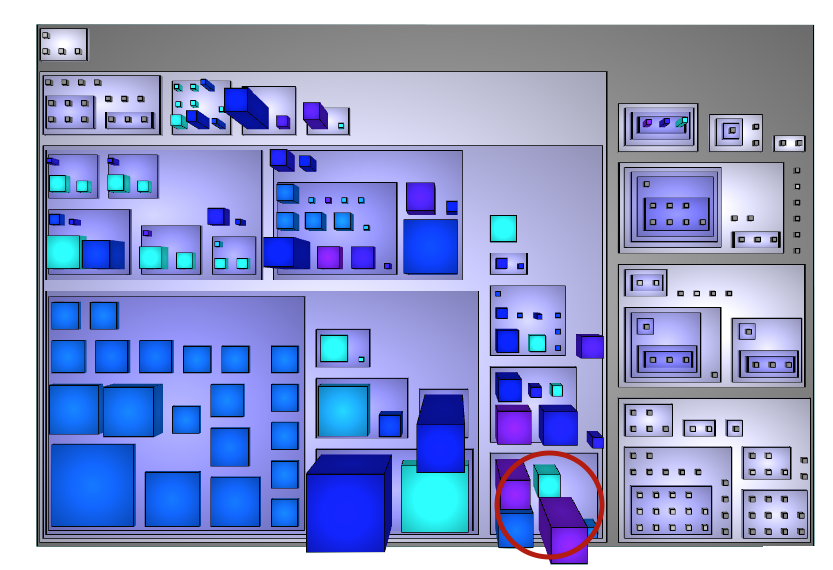
\includegraphics[width=.45\textwidth,height=4cm,keepaspectratio]{images/discPer}
\label{fig:per:a}
}
\hspace*{\fill}
\subfigure[Percentage]{
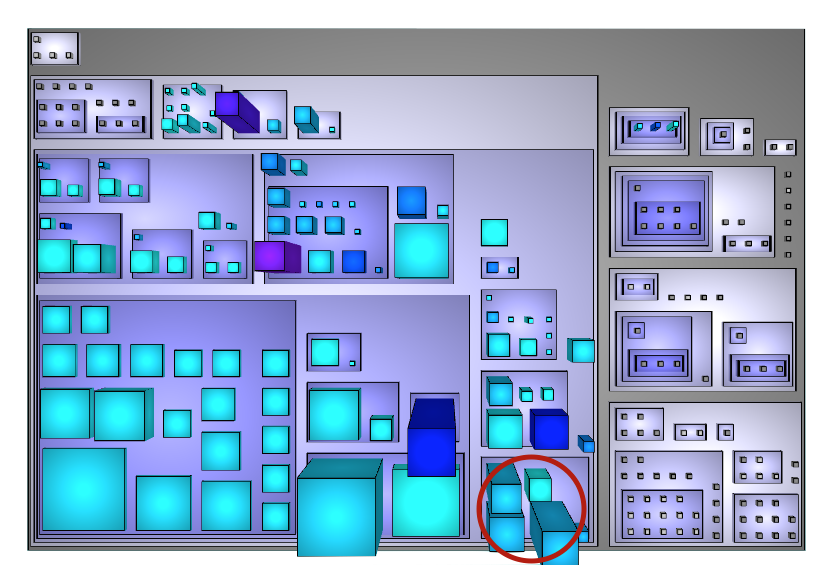
\includegraphics[width=.45\textwidth,height=4cm,keepaspectratio]{images/discAbs}
\label{fig:per:b}
}

\caption{Colors Absolute \& percentage}
\label{fig:per}
\end{figure}
Figure \ref{fig:per}  depicts two different color options, absolute in Figure \ref{fig:per:a} and percentage Figure \ref{fig:per:b}.
It is interesting to note that there are some buildings that have the majority of discussions in the absolute view (colored in purple) and at the same time the method has not complete information coverage (in percentage View). An example is circled in Figure \ref{fig:per}. 


\subsubsection{Code related Colour meaning}






The color used to compute the code related information represents  the number of methods, fields, classes or interfaces in files. It is useful to check the code style, for example the number of classes or interfaces in a file, or to get an idea where the majority of the methods and fields are concentrated. The scale is the same as above: purple means the maximum amount of  data and light blue no data available.

Figure \ref{fig:classAbs} shows an example in which the colors represent the number of classes in the project. Here, there are a lot of files that contains only one class and only a few files that contains more then one class. 
	

 \begin{figure}[H]
	\centering
	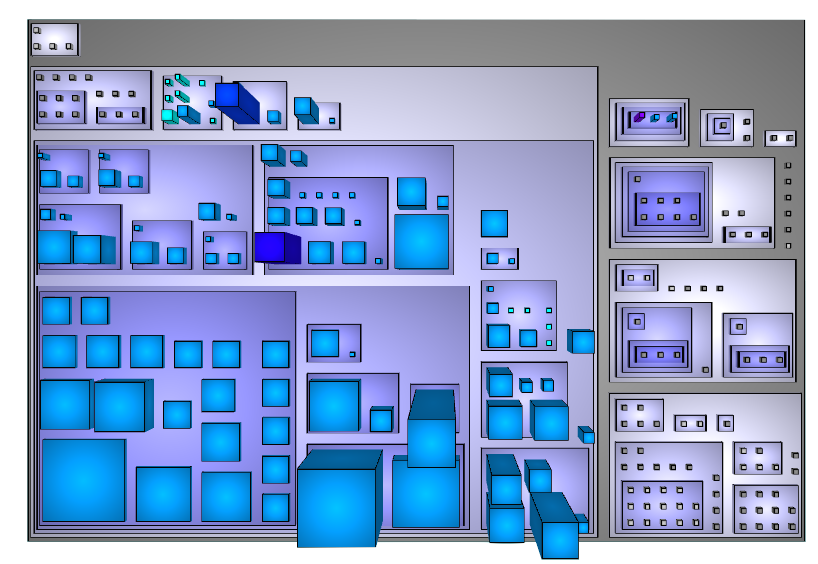
\includegraphics[width=0.95\textwidth]{images/classAbs}
	\caption{Absolute number of class \label{fig:classAbs}}
 \end{figure}





\subsection{System architecture }
The project is divided in to two different parts. The \stormed importer that imports into the database all the useful data from the \stormed Dataset and the visualizer that is the part that allows the developers to navigate, interact and modify the city. The former part is written in Scala and latter in Java using the Play Framework. The application is web based. 




\subsubsection{\stormed importer}
\stormed importer is nothing else than a visitor of a JSON file that represent a discussion. The JSON file contains an H-AST of the discussion whit all the information. Since we need only a small subset of this information, we extract the useful one, such as method calls with the number of parameters and the imports, and we store it in the database. Since this operation is time-consuming, we adopt a multi-thread solution that reduces drastically the time used to analyze all the files. Only to give an idea, we keep approximately several hours on a server with 56 Intel 2.10 Ghz Xeon processor and 300 GB of RAM.

The script that deals with this is written in Scala combined with a database query and access library called \textit{Slick}\footnote{http://slick.lightbend.com/}.


\subsubsection{Visualizer}
The visualizer is the core of the system. Since it is a web application, it consists of a back-end and a front-end part. All the computation is done on the server side since the amount of data is large; we also choose a strategy to precompute the main metrics and store them as JSON files.
The process is represented in  Figure \ref{fig:processPipeline}.


\begin{figure}[ht]
	\centering
	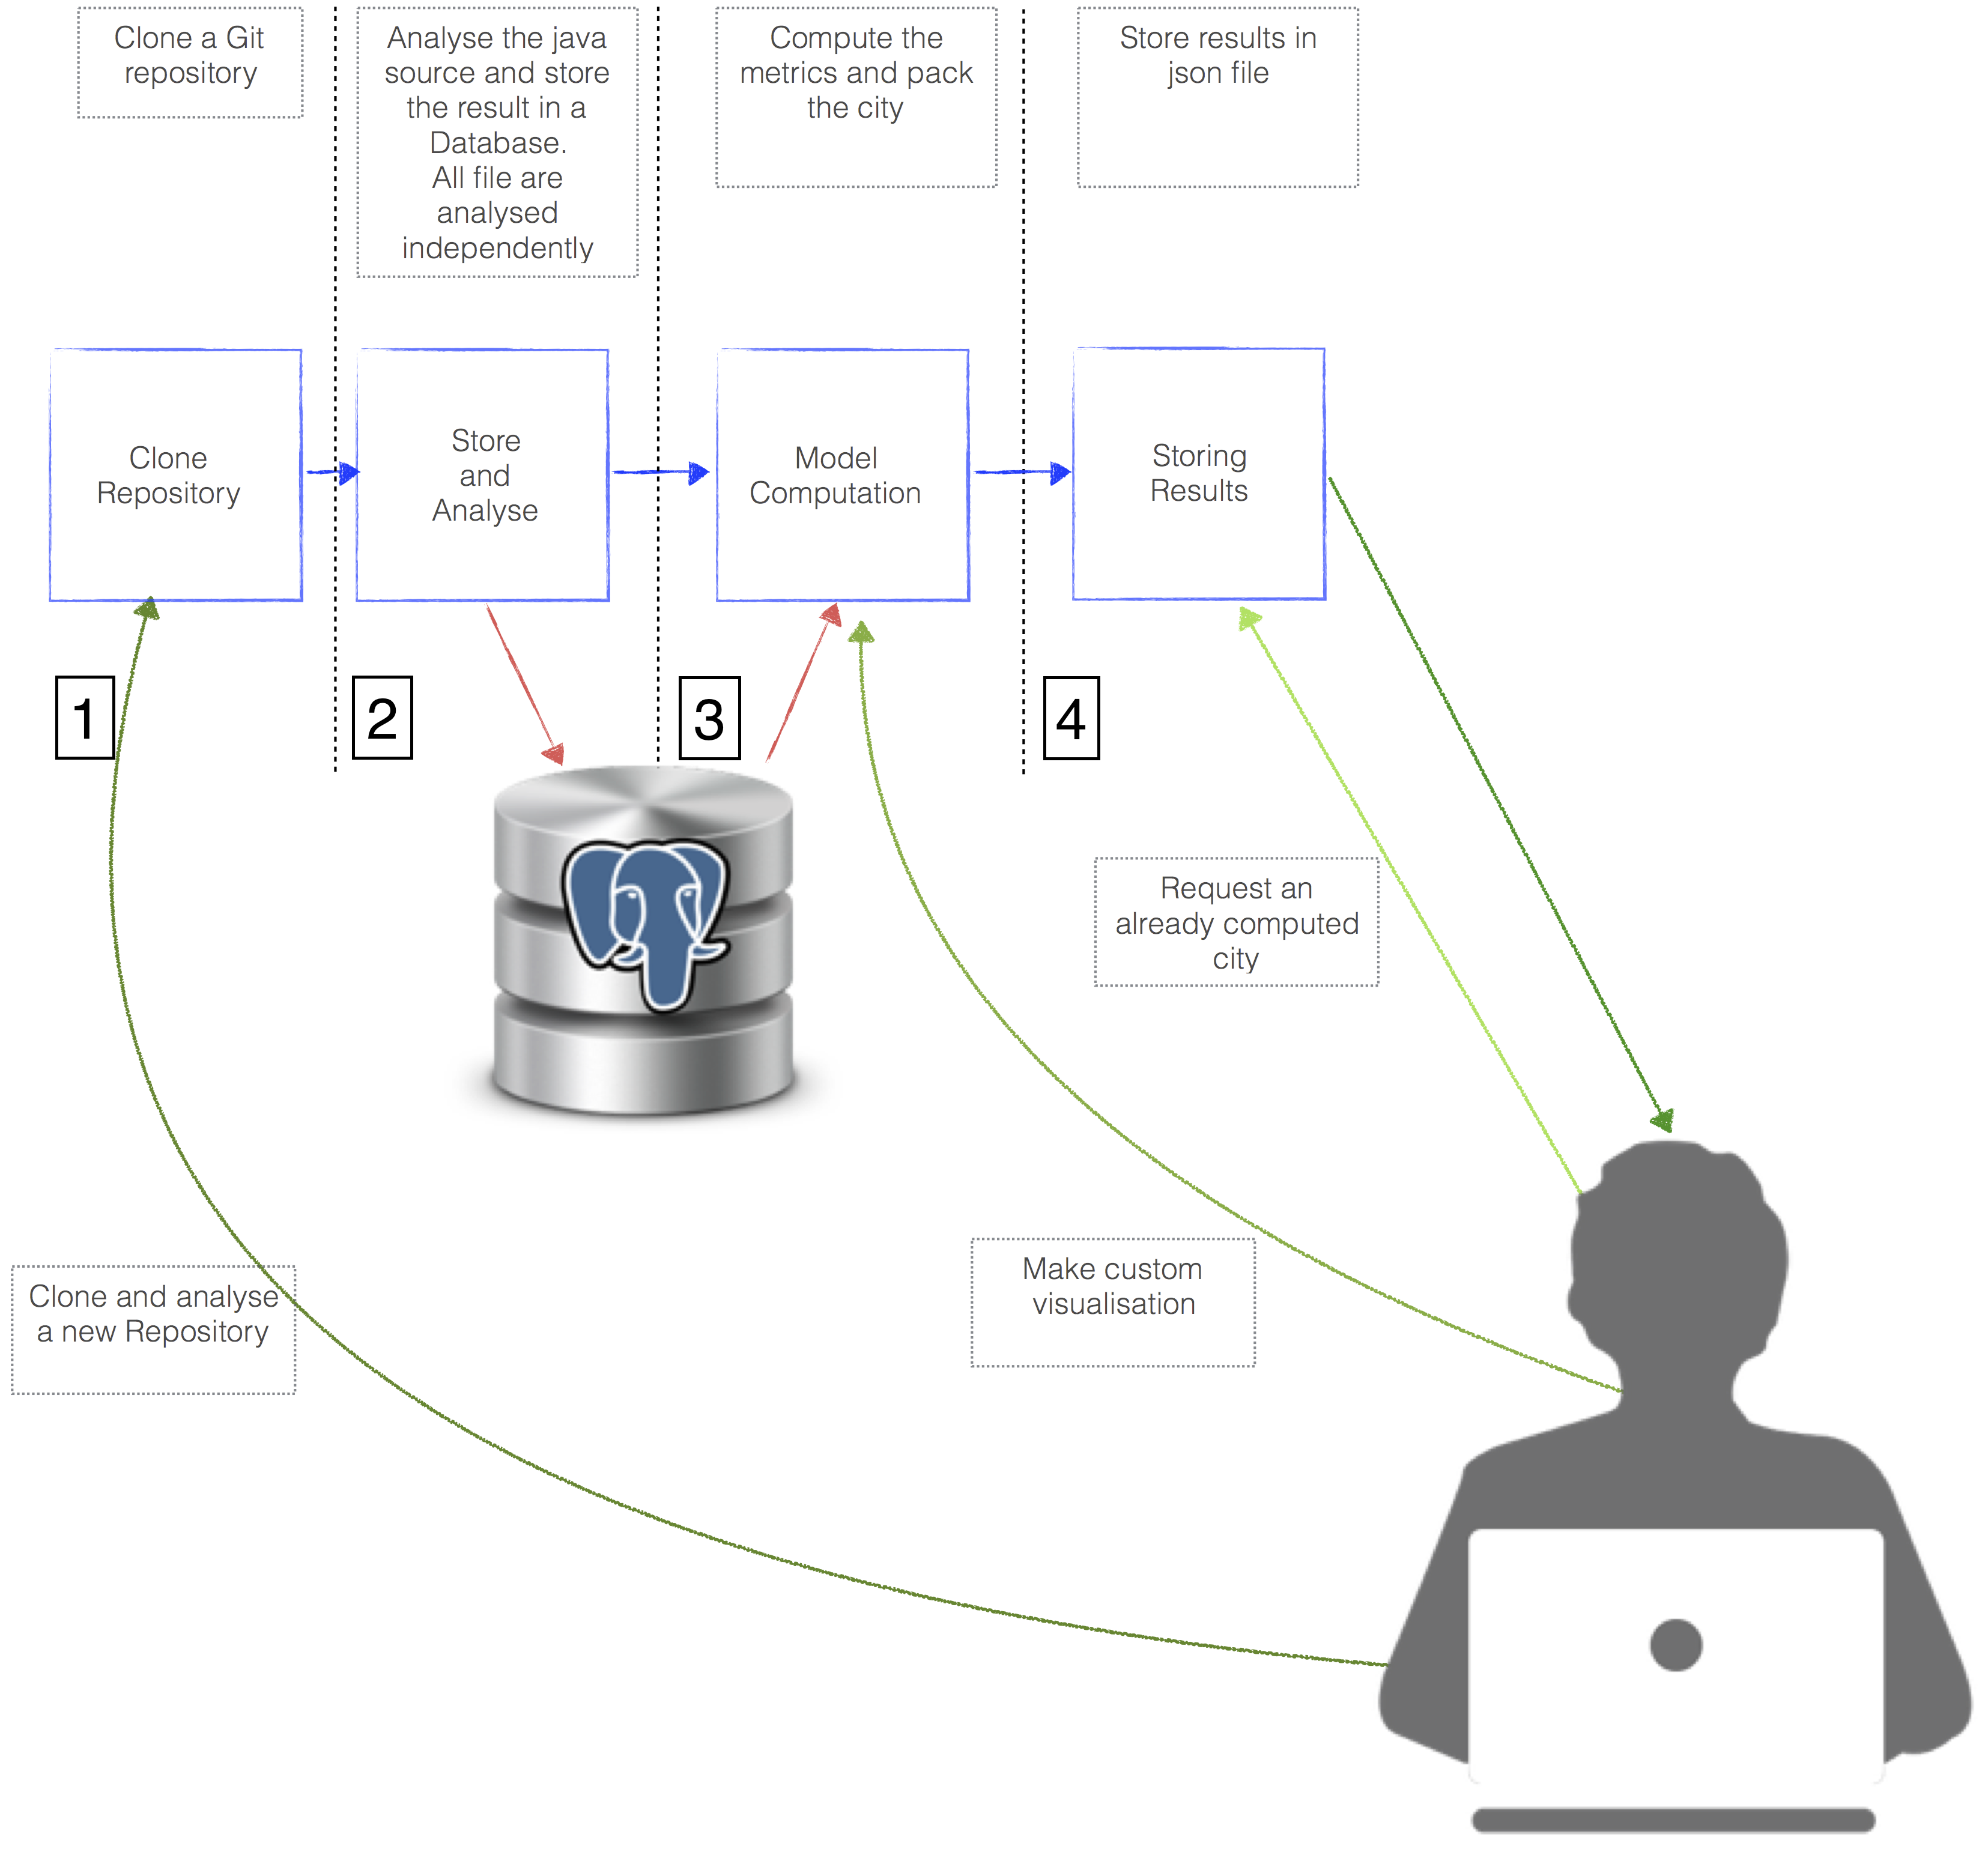
\includegraphics[width=0.45\textwidth]{images/processPipeline}
	\caption[Process Pipeline]{Process Pipeline\label{fig:processPipeline}}
\end{figure}

The process is as follows:

\begin{enumerate}

\item Upload the repository. We use a git subversion system. User have to provide the URL of their git repository and then insert their account information.

\item Files analysis. We traverses the directory of the repository and model an AST for each java file. This process writes into the database all the file characteristics such as classes, methods interfaces and fields(represented as red arrows).

\item Generate the city. All the actions employed at this stage are functions applied to each node in the tree. The first pass through the tree is the size computation, that gives to each node the value for width, height, and color. Since the project structure is a tree, we maintain this structure during all the process. To improve the performance during the visualization, we generate one city for each different metric computation.
The packing algorithm is done as if each package reside in the origin of the axes. Only during the rendering time we move the package around the scene.
\item Store the result in a JSON file. This file contains a tree whit all the information of the render. To obtain extra information like the list of the discussions or the file contents we need to execute some database queries( all possible user interaction are show with green arrows).

\end{enumerate}

We give to the user also the opportunity to make his own city, by deciding through a predefined list of metrics which assign to each dimension. This process repeat exactly the same passages done after the AST. Note that we also cache the result for future requests. 
The front end part gives to the user a way to interact whit the system. The most interesting part is the rendering of the JSON: the root of the city is draws at the origin and at each recursion we assign a new origin in which the package should be drawn.
We also implement a small query system that gives a way to search file or package in the city. By double clicking on a building, it appears a pop-up with the java code and we highlight the keyword to made the code readable. Also, there is a list of discussion views.
All the back end is written using \textit{Play Framework}\footnote{https://www.playframework.com/} and Java.  For the front end we use \textit{bootstrap}\footnote{http://getbootstrap.com/} and ES6 with \textit{webpack}\footnote{https://webpack.github.io/} plus the babel parser \textit{Babylon}.
We use \textit{Babylon.js}\footnote{http://www.babylonjs.com/} as 3d engine that works on top of \textit{WebGl}. Since we are on a browser, we can not have more than 10k of boxes. 






   





\newpage

\section{Use cases} \label{evaluation}

\subsection{Introduction}
In this section we are going to analyse two projects by using our tool. 
The analysis of this project is split in two parts. The former part concern the structure, in which we are looking for code identity harmony (See Section \ref{sec:idHarmony}). In the latter part we analyse the information coverage. 

For the former part we can not say that a particular design is wrong, we could only give a monitor to the developers to check some port and understand if it is correct.
A virtual demo is available on \url{http://rio.inf.usi.ch:51001/}: it is possible navigate and play with these two projects. 

\subsection{Use case I: Tomcat}
The Apache Tomcat\footnote{http://tomcat.apache.org/} software is an open source implementation of the Java Servlet, JavaServer Pages, Java Expression Language and Java WebSocket technologies. 
The Apache Tomcat software is developed in an open and participatory environment. The Apache Tomcat project is intended to be a collaboration of the best-of-breed developers from around the world.

\subsubsection{Code related analysis}

Figures \ref{fig:tomcat:a} and \ref{fig:tomcat:b}  depict Tomcat's code related information. The buildings represent the java files post on top of his package. The height of a building is the number of methods and the width is the number of fields. The color represents the number of interfaces (Figure \ref{fig:tomcat:b}) and  the number of classes (Figure  \ref{fig:tomcat:a}).
Generally, we have an equal distribution of class and interface for each file, there are only a few disharmony.

\begin{figure}[H]
	\centering
	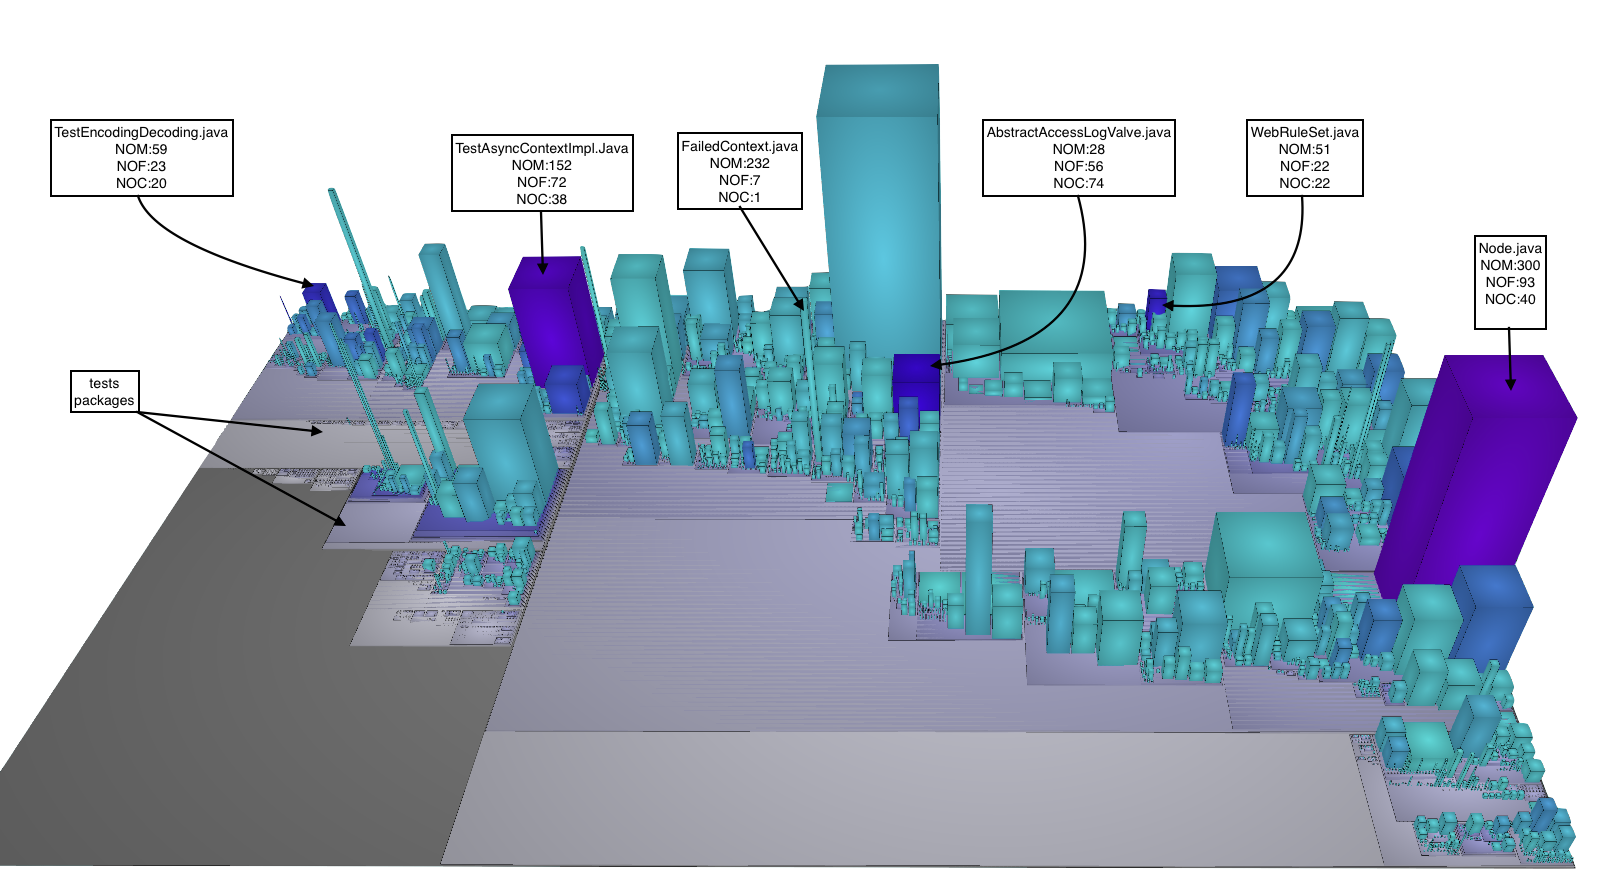
\includegraphics[width=0.95\textwidth]{images/tomcatClss}
	\caption[Tomcat: Classes ]{Tomcat:  The color represent the classes distribution \label{fig:tomcat:a}}
\end{figure}



          

In Figure \ref{fig:tomcat:a} there are some classes that have a high concentration of inner classes. The file has a huge number of private static classes. This is not a problem for the Java Code Conventions \cite{oracle}: there is not more than one public class and all the other inner classes are inside the public class. The names and the characteristics are shown in the figure. Two of them are test classes, the other three are not. The test classes are fine. The other three classes could have a high level of coupling that is a hint to check the design. Regarding the interface, we have some files that contain more than one. In this case, we have not a big number of interfaces, so it could be a design choose and not a problem.
Now we take a look at the methods and fields of a class. As we can expect, the class \textit{Node.java} has a lot of methods but at the same time it has a huge number of classes as showed before. It is a good candidate for a God Class. \textit{StandardContex.java} has the potential to be a God Class either, since it has only three classes and a huge number of methods and fields. In both classes, we can find in a high level of coupling.

\begin{figure}[H]
	\centering
	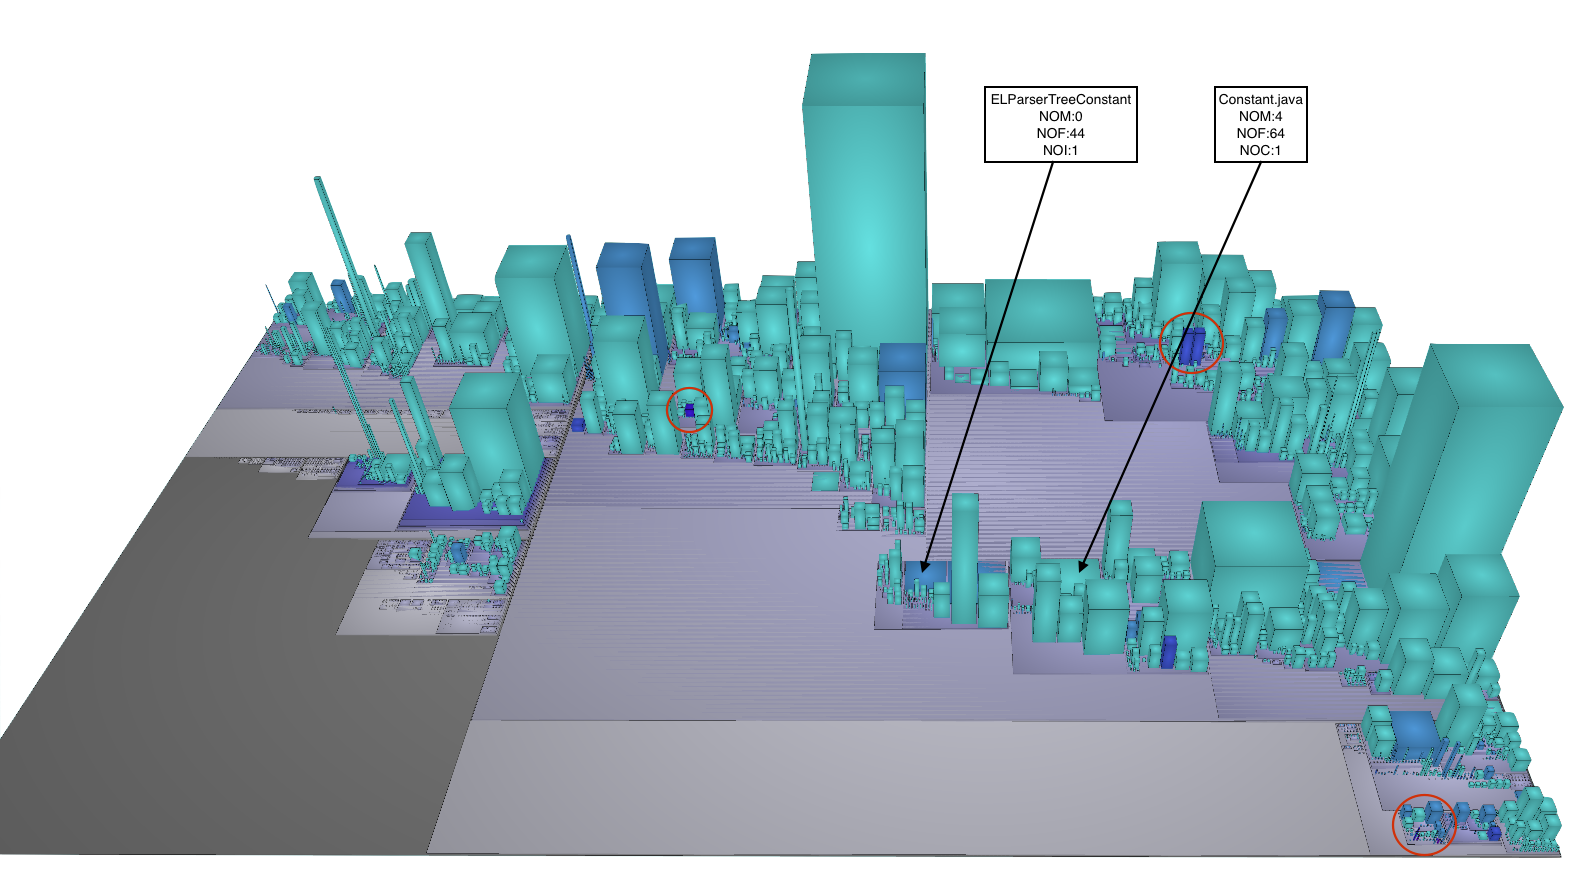
\includegraphics[width=0.95\textwidth]{images/tomcatInt}
	\caption[Tomcat: Interfaces]{Tomcat:  The color represent the interfaces distribution \label{fig:tomcat:b}}
\end{figure}

There are a few buildings that look like a Brain Class. We do not care about test classes since they are, by definition, a list of methods. The first one is  \textit{FailledContext.java}, that has a huge amount of methods and no too much fields. In Figure \ref{fig:tomcat:a} there are other classes of this type.
The Data Classes are not too much, one is \textit{Constant.java} and there are others shown in Figure \ref{fig:tomcat:b}.



\subsubsection{Corollary information analysis}





\begin{figure}[H]
	\centering
	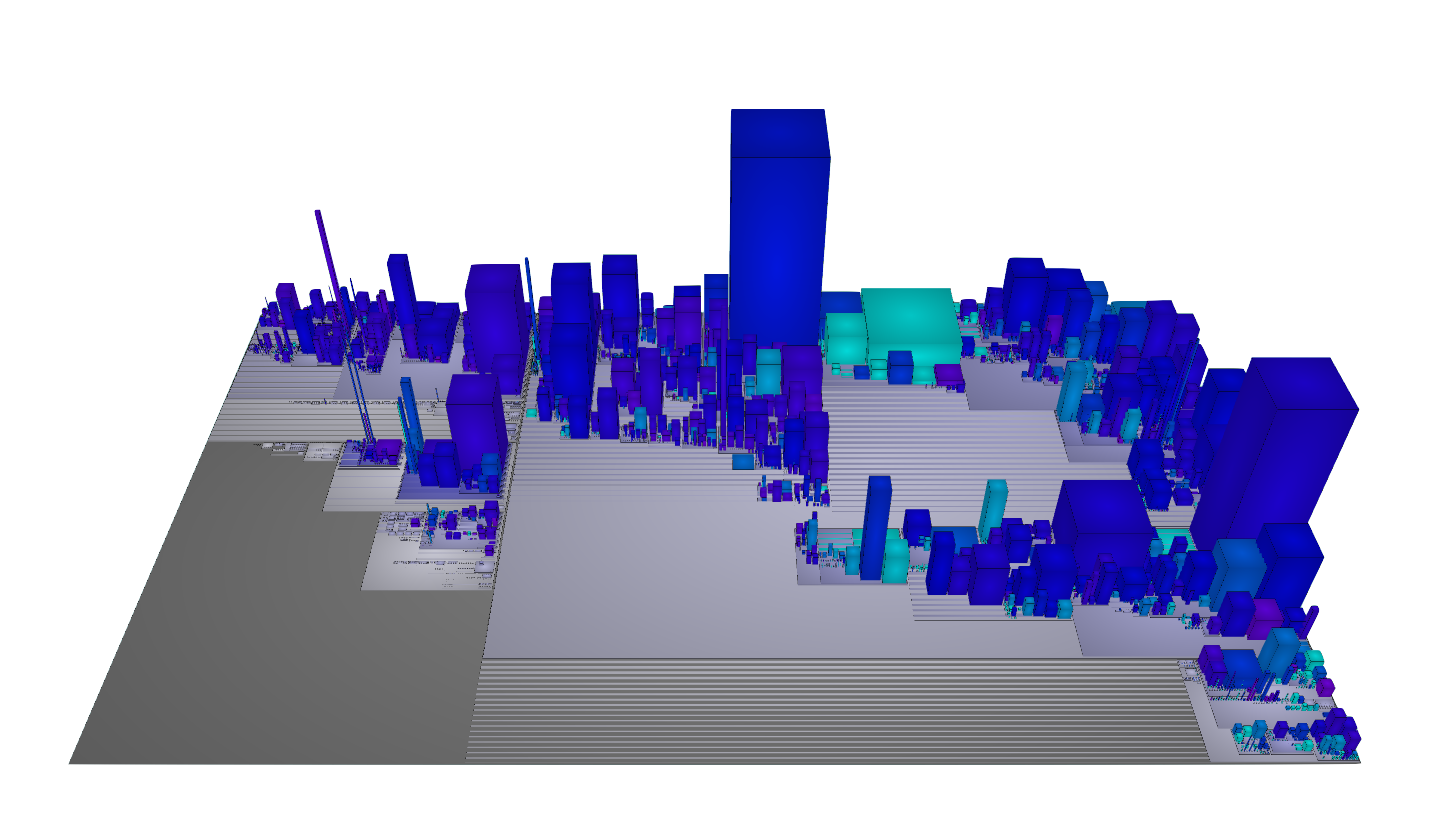
\includegraphics[width=0.95\textwidth]{images/discussionTomcat}
	\caption[Tomcat: Discussions ]{Tomcat: The color represent the interfaces  distribution  \label{fig:tomcatCorrollary:a}}
\end{figure}





Figure \ref{fig:tomcatCorrollary} depicts the information related to the code of the Tomcat repository. The buildings represents the java files post on top of their packages. The height of a building is the number of methods and the width is the number of fields. The color represents the number of discussions over method calls (Figure \ref{fig:tomcatCorrollary:a}), the amount of java documentations over method declarations (Figure \ref{fig:tomcatCorrollary:b}) and the information coverage (Figure \ref{fig:tomcatCorrollary:c}).

\begin{figure}[H]
	\centering
	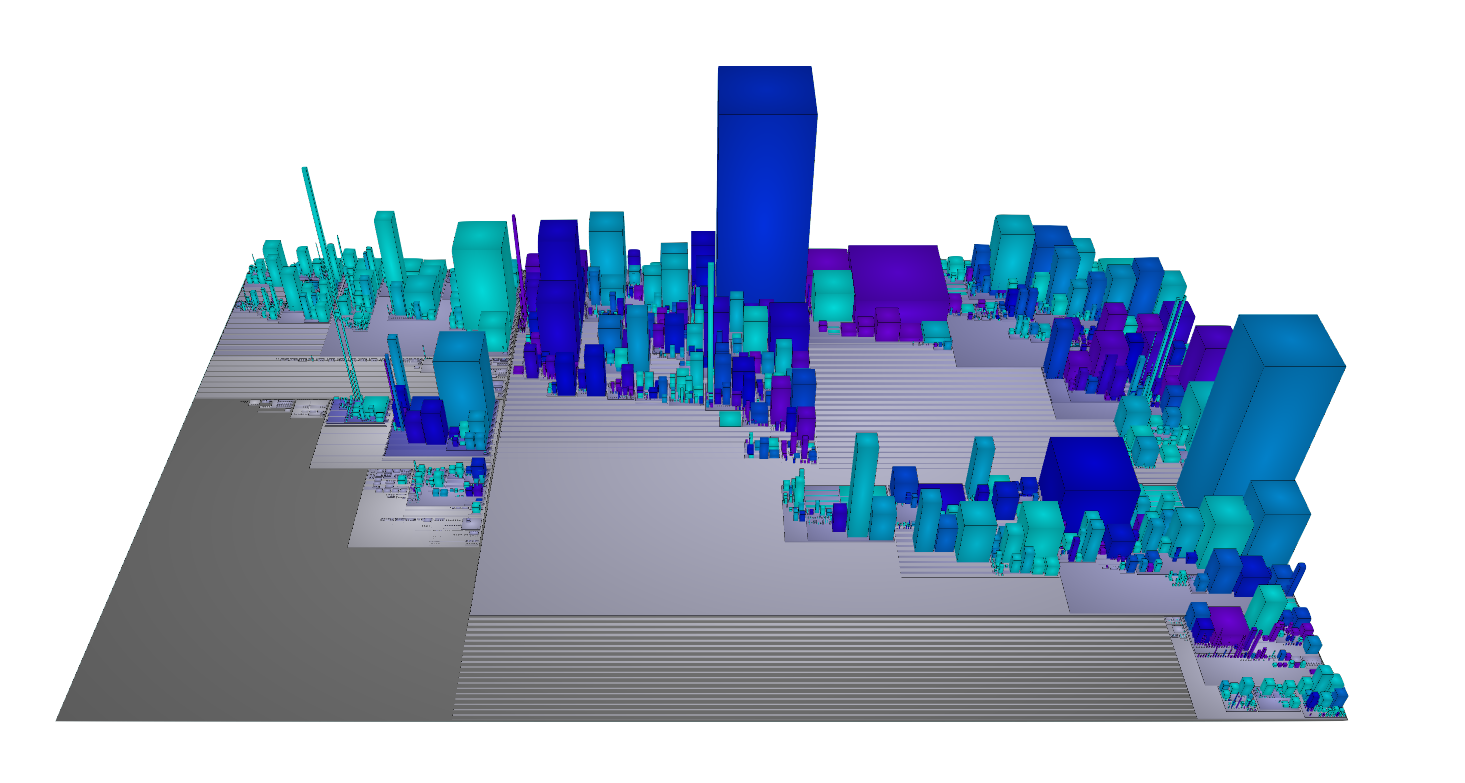
\includegraphics[width=0.95\textwidth]{images/javadocTomcat}
	\caption[Tomcat: Java Documentation]{Tomcat: The color represent the Java Documentation distribution \label{fig:tomcatCorrollary:b}}
\end{figure}

Let's start analyze the java documentation: there are classes completely documented and others that have not documentation at all.
The tests are completely not documented and some of the classes that have more methods, have a lower percentage of documentation. This part should be better documented.
Instead, the discussion coverage is pretty good. The color of the city in average is dark blue and there are a lot of building purple this means a lot of discussions related to the code. 
Now that we have the result of both metrics we can merge it together and we have the Figure \ref{fig:tomcatCorrollary:c}. Thanks to the discussions found online and the code documentations, the the system has a homogeneous information coverage.
\begin{figure}[H]
	\centering
	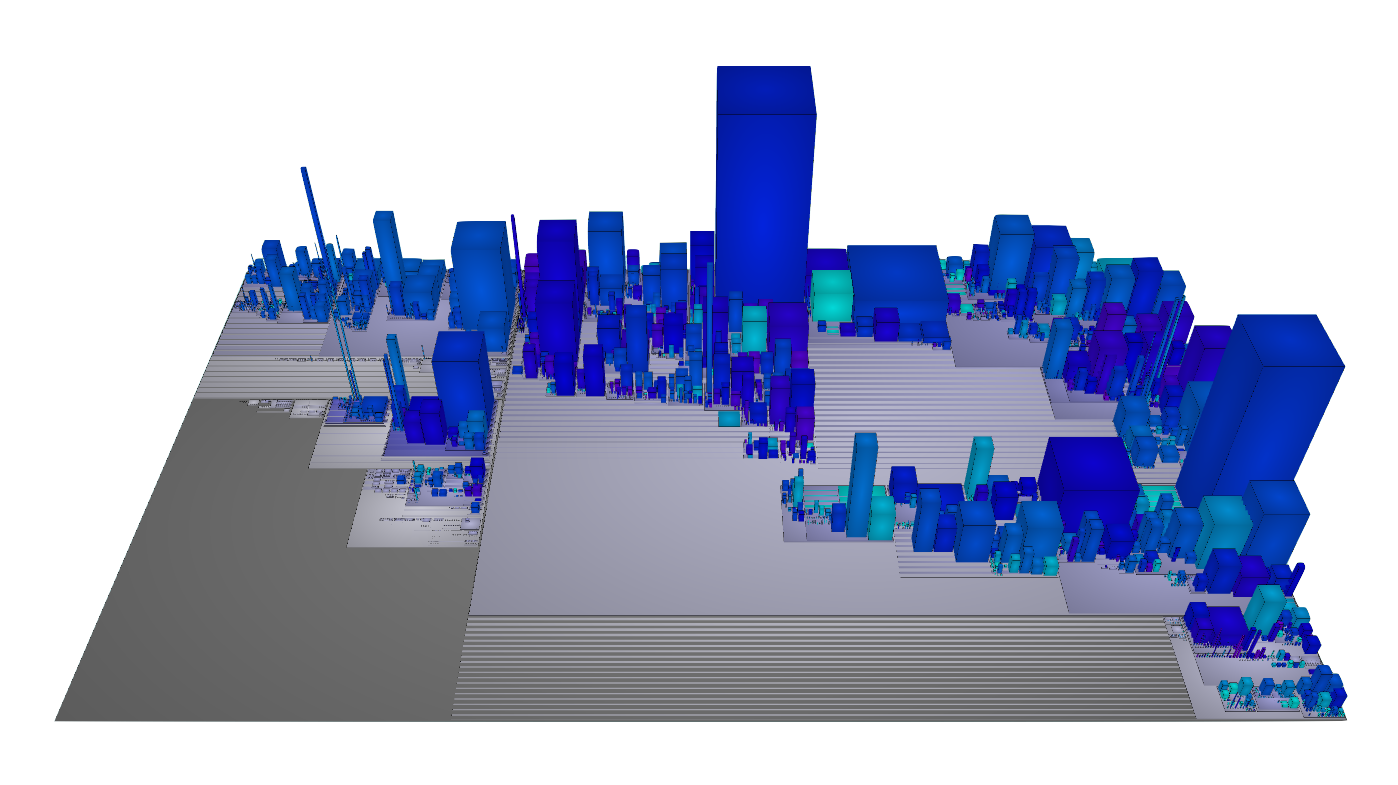
\includegraphics[width=0.95\textwidth]{images/javaDocAndDiscussionTomcat}
	\caption[Tomcat: Discussion and Java Documentation]{Tomcat: Discussion and Java Documentaton \label{fig:tomcatCorrollary:c}}
\end{figure}


 

\newpage



\subsection{Use case II: JGit}
JGit\footnote{https://eclipse.org/jgit/} is an implementation of the git version control system for java. We analyse the system in the same way as for Tomcat. We decided to use this system since is also used in Cub8. It is an example of an open source product and it is also part of the Eclipse IDE\footnote{https://eclipse.org/}.


\subsubsection{Code related analysis}


			
\begin{figure}[H]
	\centering
	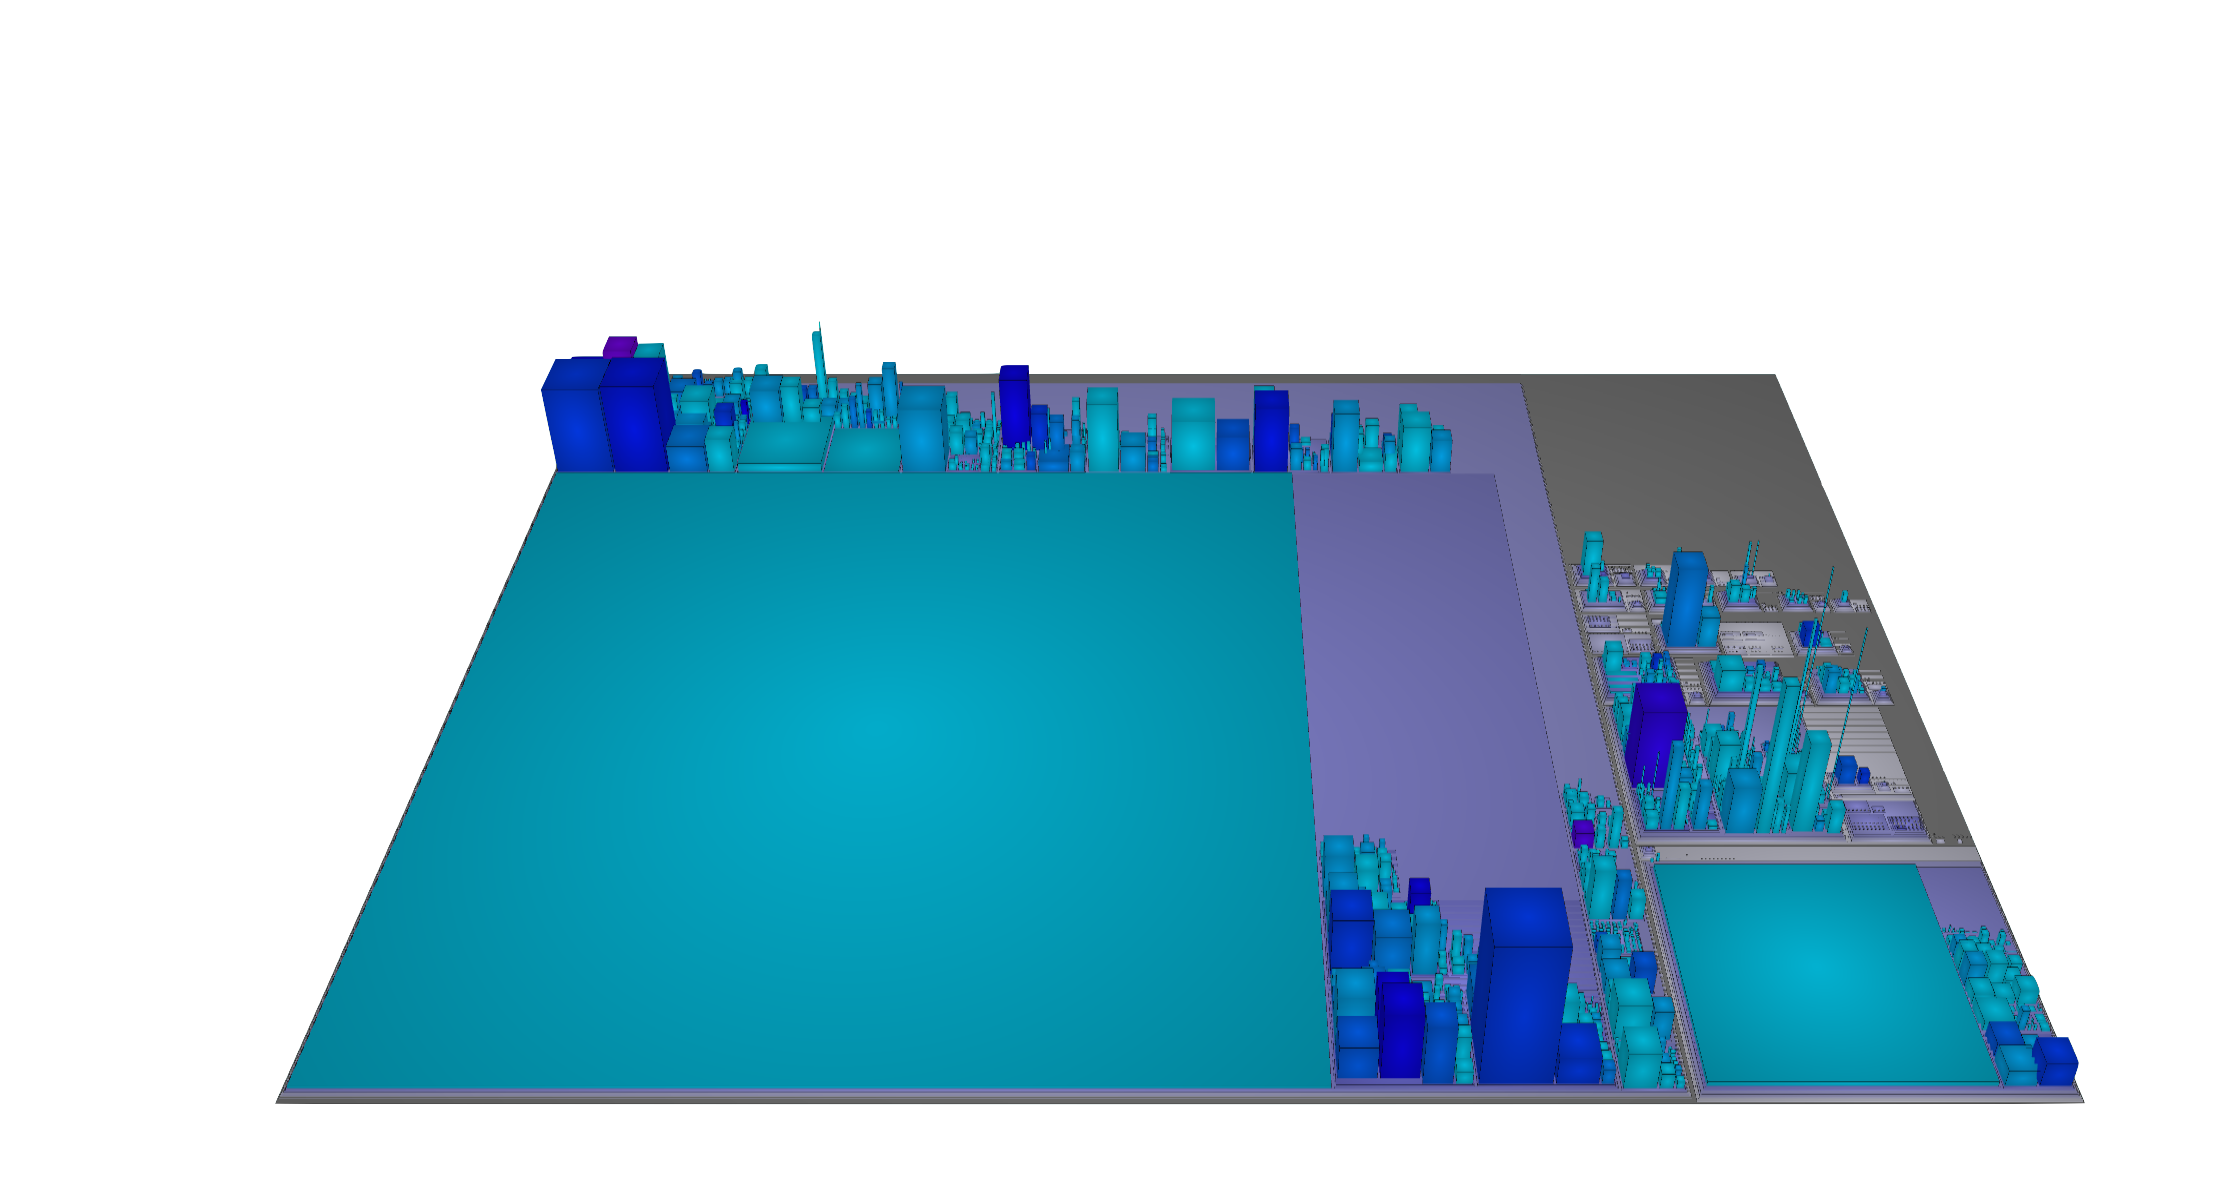
\includegraphics[width=0.95\textwidth]{images/jgitClass}
	\caption[JGit: Classes]{JGit:  The color represent the classes distribution \label{fig:jgitRel:a}}
\end{figure}





Figures \ref{fig:jgitRel:a}  and \ref{fig:jgitRel:b}  depicts JGit's code related information. The height of a building is the number of methods and the width is the number of fields. The color, in Figure \ref{fig:jgitRel:a}, represents the number of classes, in Figure \ref{fig:jgitRel:b} the number of java interfaces.


\begin{figure}[H]
	\centering
	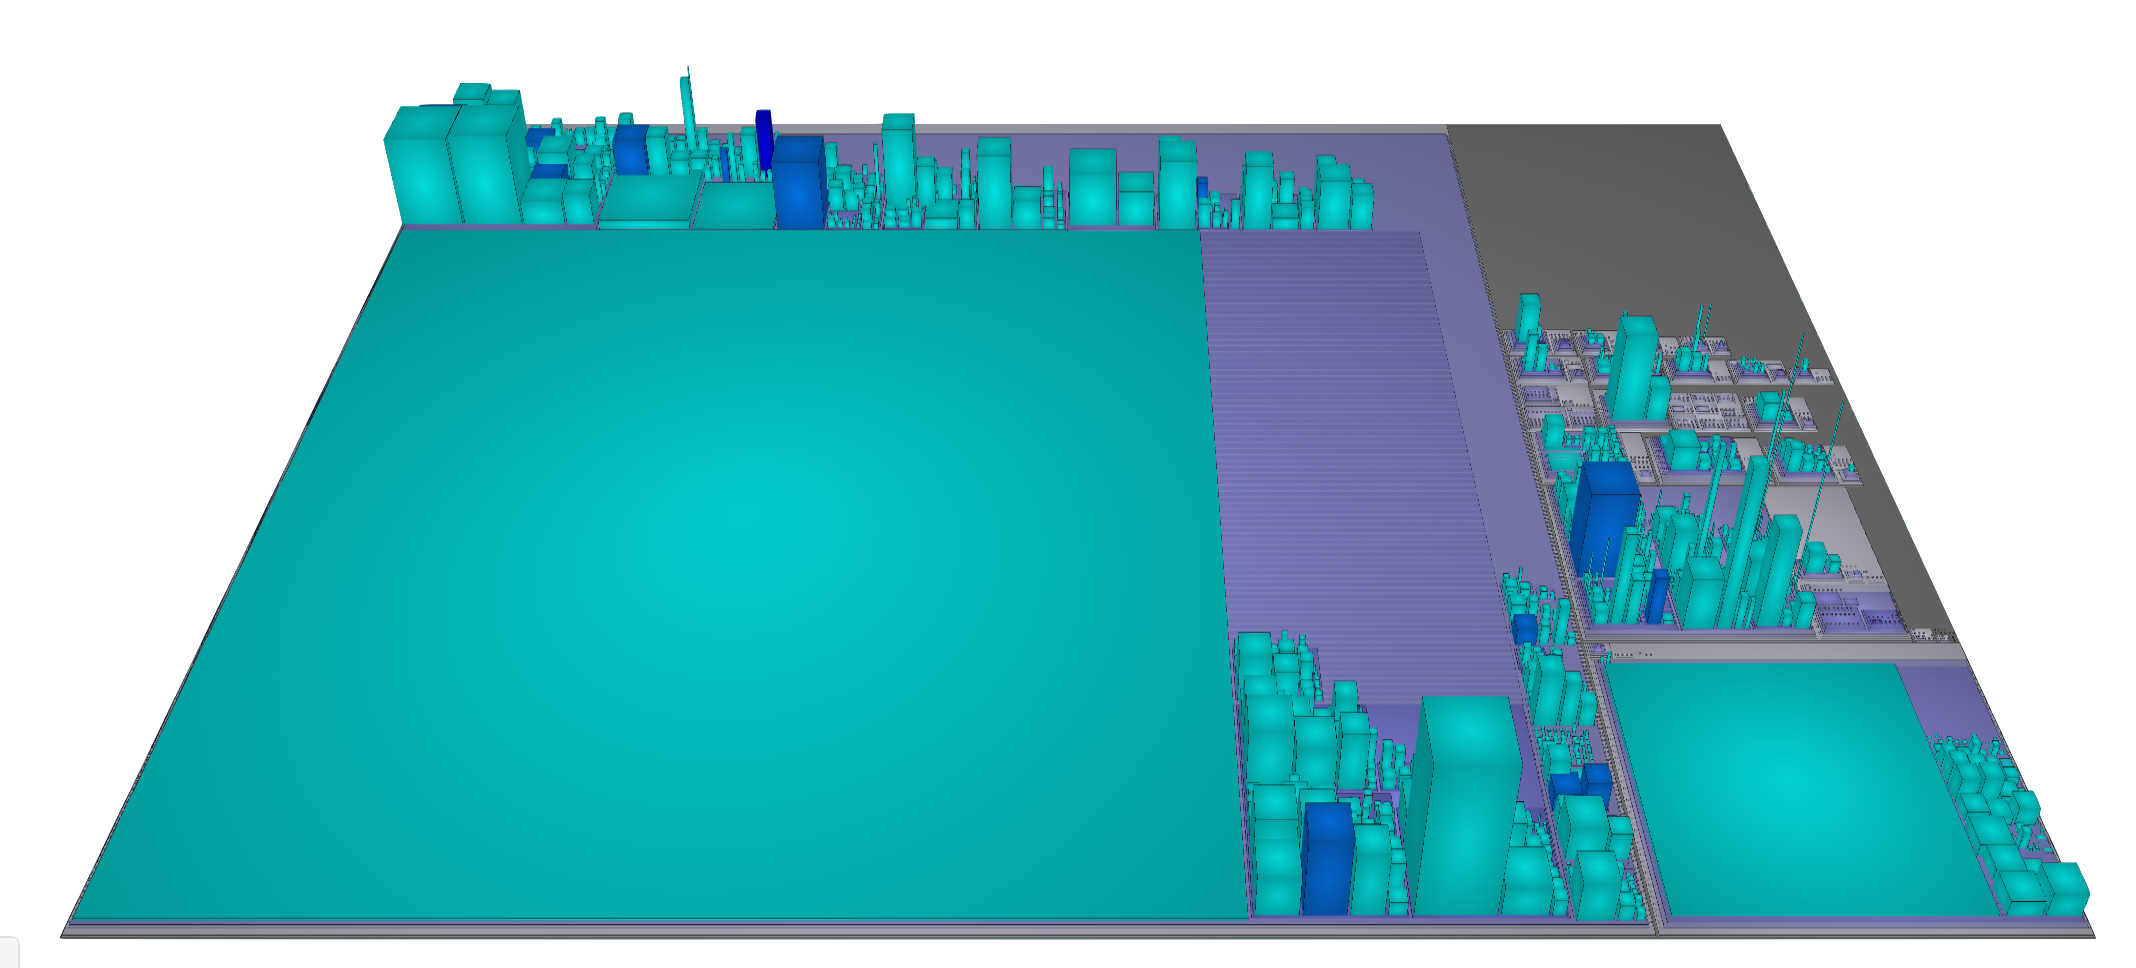
\includegraphics[width=0.95\textwidth]{images/jgitInterface}
	\caption[Jgit: Interfaces]{JGit: The color represent the interfaces distribution. \label{fig:jgitRel:b}}
\end{figure}


The classes view (Figure \ref{fig:jgitRel:a}), shows that there are some files that have more than one classes. It os important to note that the maximum amount of classes for a file in this project is 10. The coupling degree is low. The interface distribution appears to be well spread, there are only few occurrences of multiple interfaces on the same file. We can see a God Class call  \textit{PackWriter.java} that has 48 fields and 121 methods. There are also two big Data Class: \textit{CLIText.java} and \textit{JGitText.java}. At last but not least there is a Brain Class call  \textit{RepositoryState.java} that has 90 methods.
 


 \subsubsection{Corollary information analysis}
 
 
 
\begin{figure}[H]
	\centering
	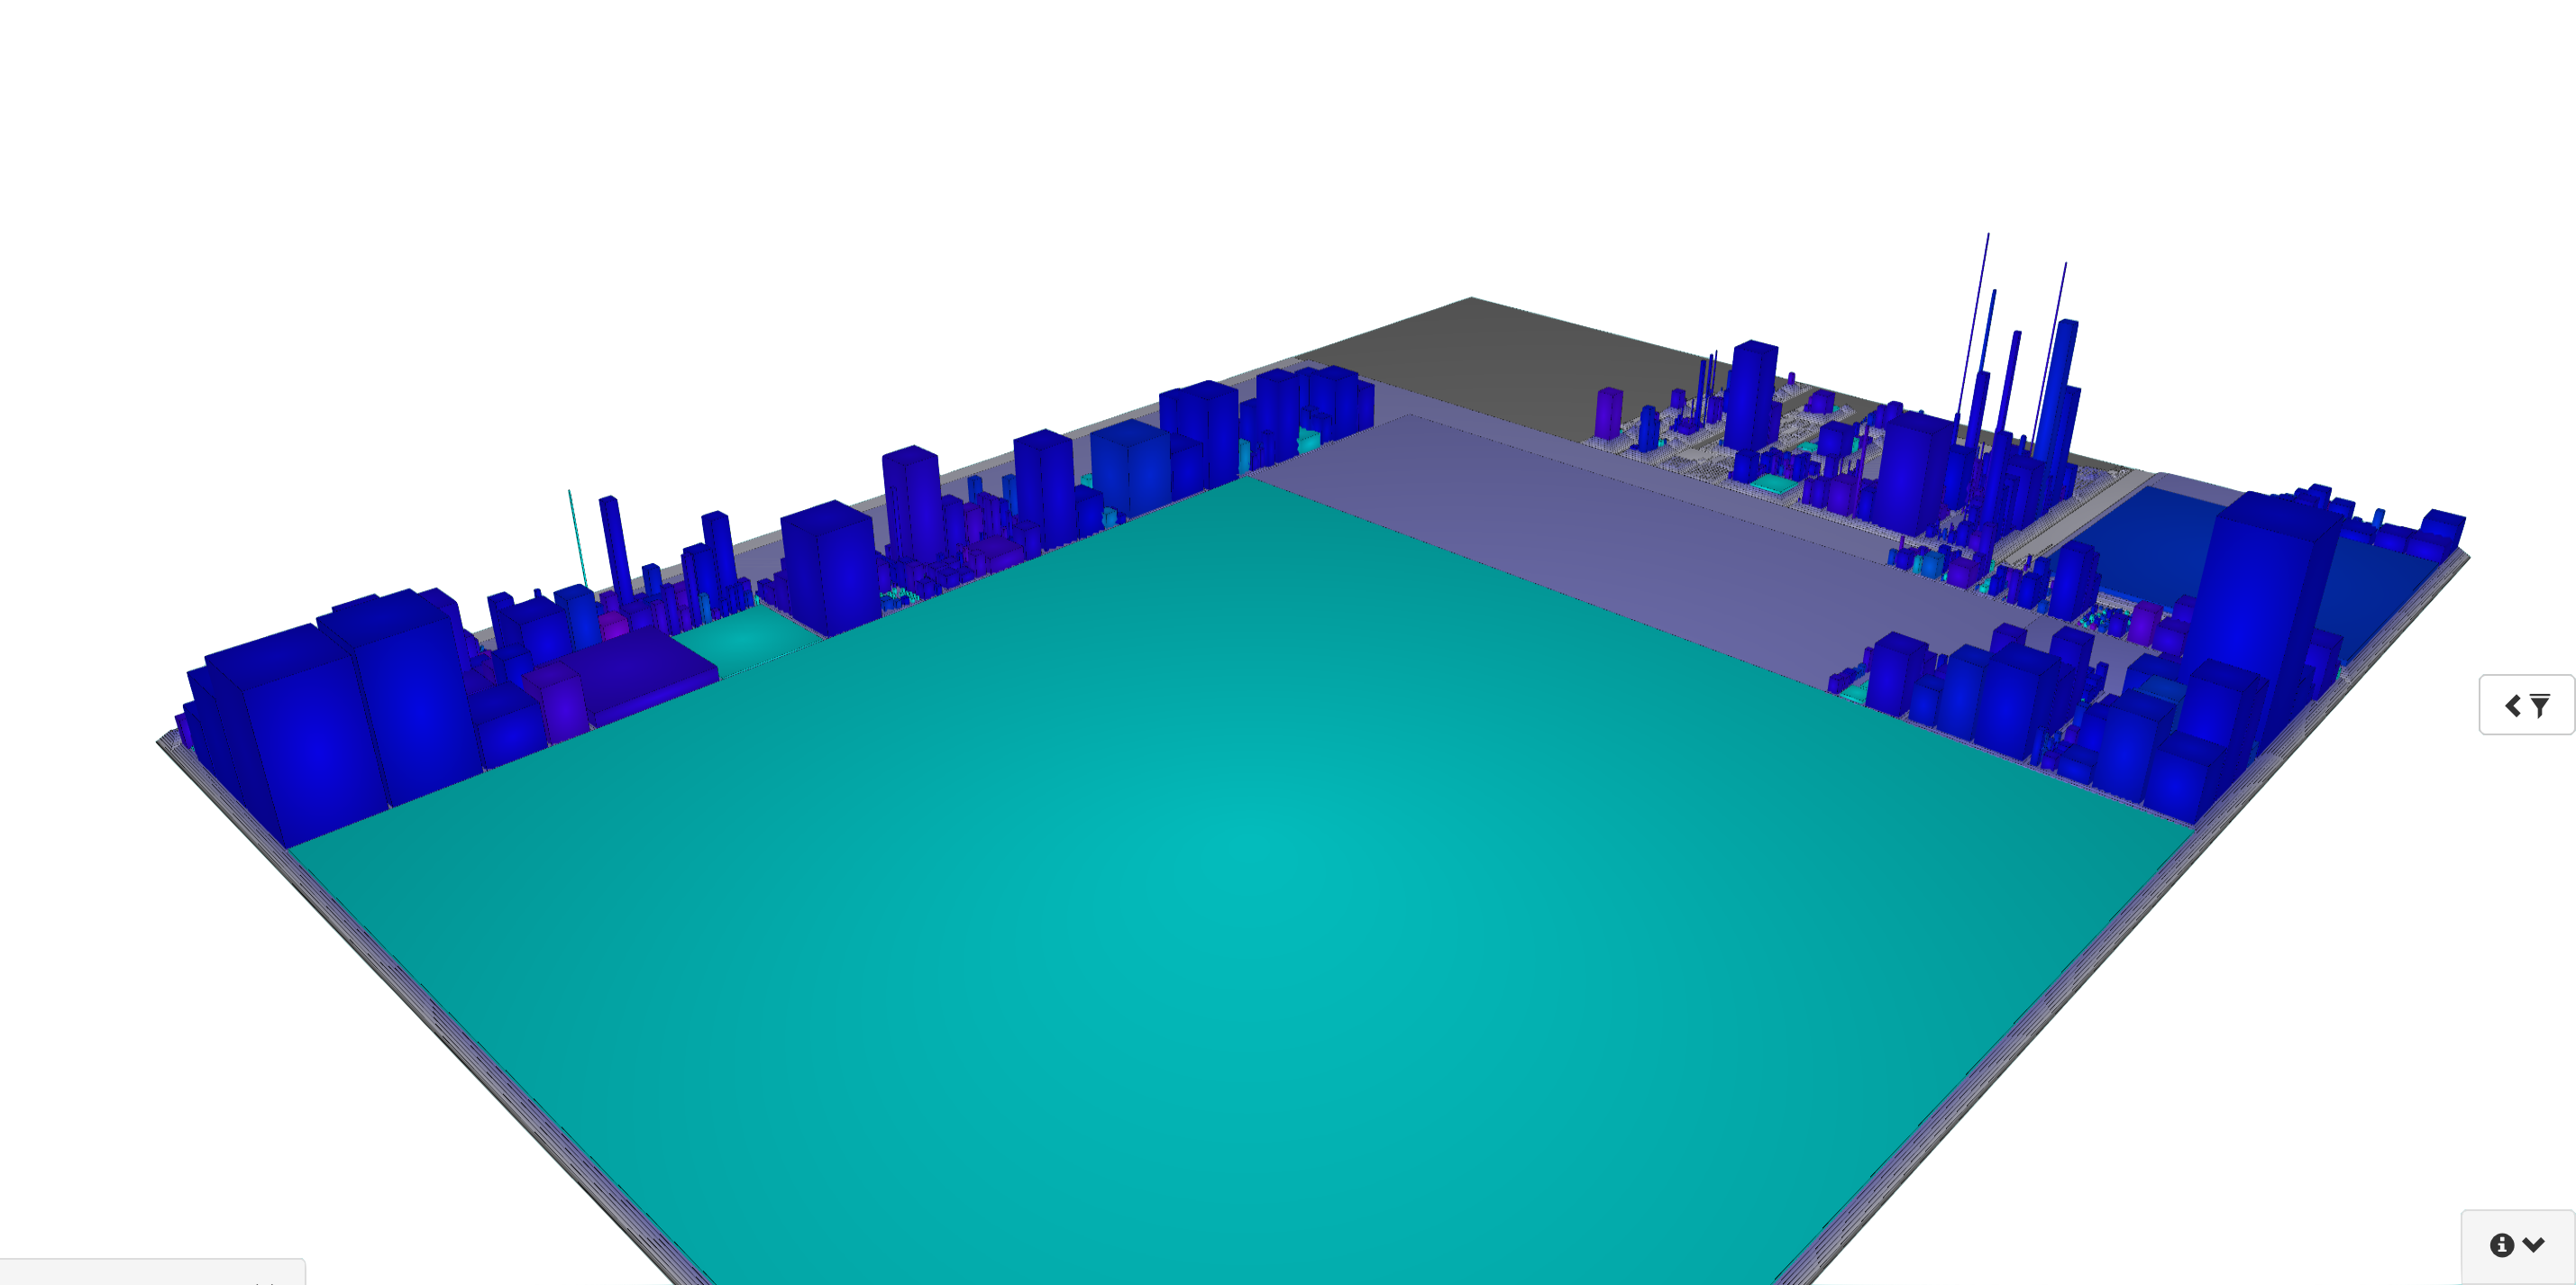
\includegraphics[width=0.95\textwidth]{images/jgitDiscussion}
	\caption[JGit: Discussions]{JGit: Discussions express in percentage respect to the number of imports and method calls \label{fig:jgitCorrollary:a}}
\end{figure}





Figures \ref{fig:jgitCorrollary:a},\ref{fig:jgitCorrollary:b} and \ref{fig:jgitCorrollary:c} depict Jgit's code corollary information. The height of a building is mapped to the number of methods and the width is mapped to the number of fields. In  Figure \ref{fig:jgitCorrollary:a} ,the color represents  the number of discussions over methods, in Figure \ref{fig:jgitCorrollary:b} the number of java documentation over methods and in Figure \ref{fig:jgitCorrollary:c} the information coverage.
\begin{figure}[H]
	\centering
	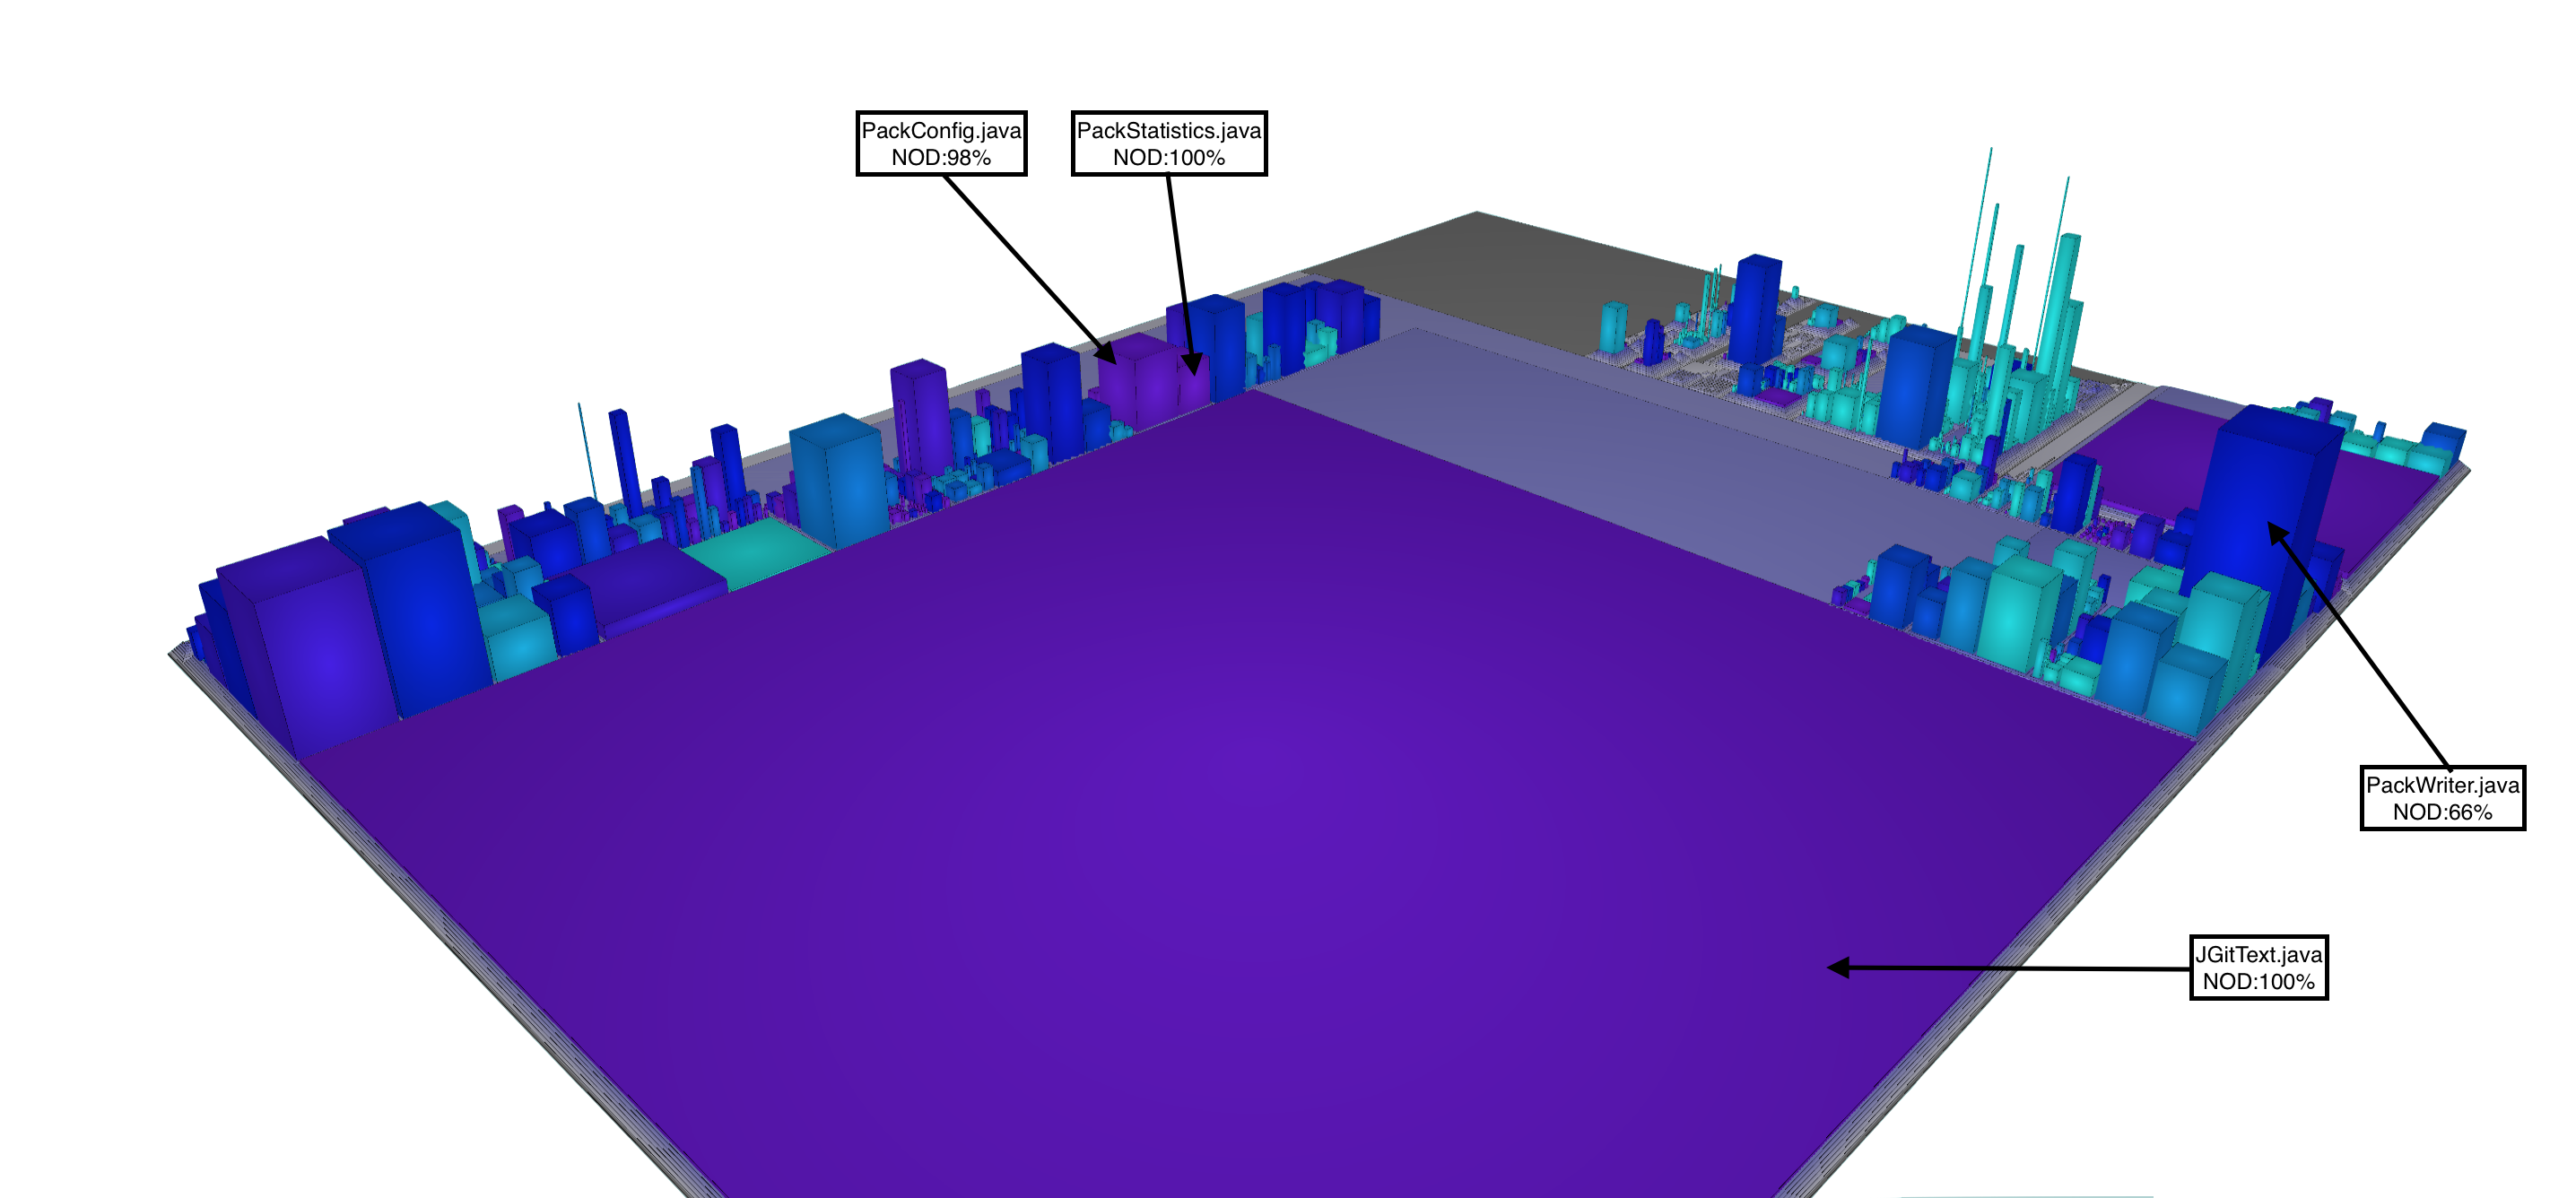
\includegraphics[width=0.95\textwidth]{images/jgitJavaDoc}
	\caption[JGit: Java Documentation]{JGit: The color represent the Java Documentation express in percentage respect to the number of methods\label{fig:jgitCorrollary:b}}
\end{figure}



Starting by Figure \ref{fig:jgitCorrollary:a} we see that the discussions available are, on average, around the 50\%. There are no discussions for JGitText, it has only one method that, the only thing that the method does it is to call another method inside the package; therefore, there are not any discussions available. There are also few classes with a 100\% of discussions coverage.
The java doc view (Figure  \ref{fig:jgitCorrollary:b}) shows that there are a lot of building without documentation. Some of them are tests, but a huge number are not and therefore a newcomer has to allocate an higher effort.  
\begin{figure}[H]
	\centering
	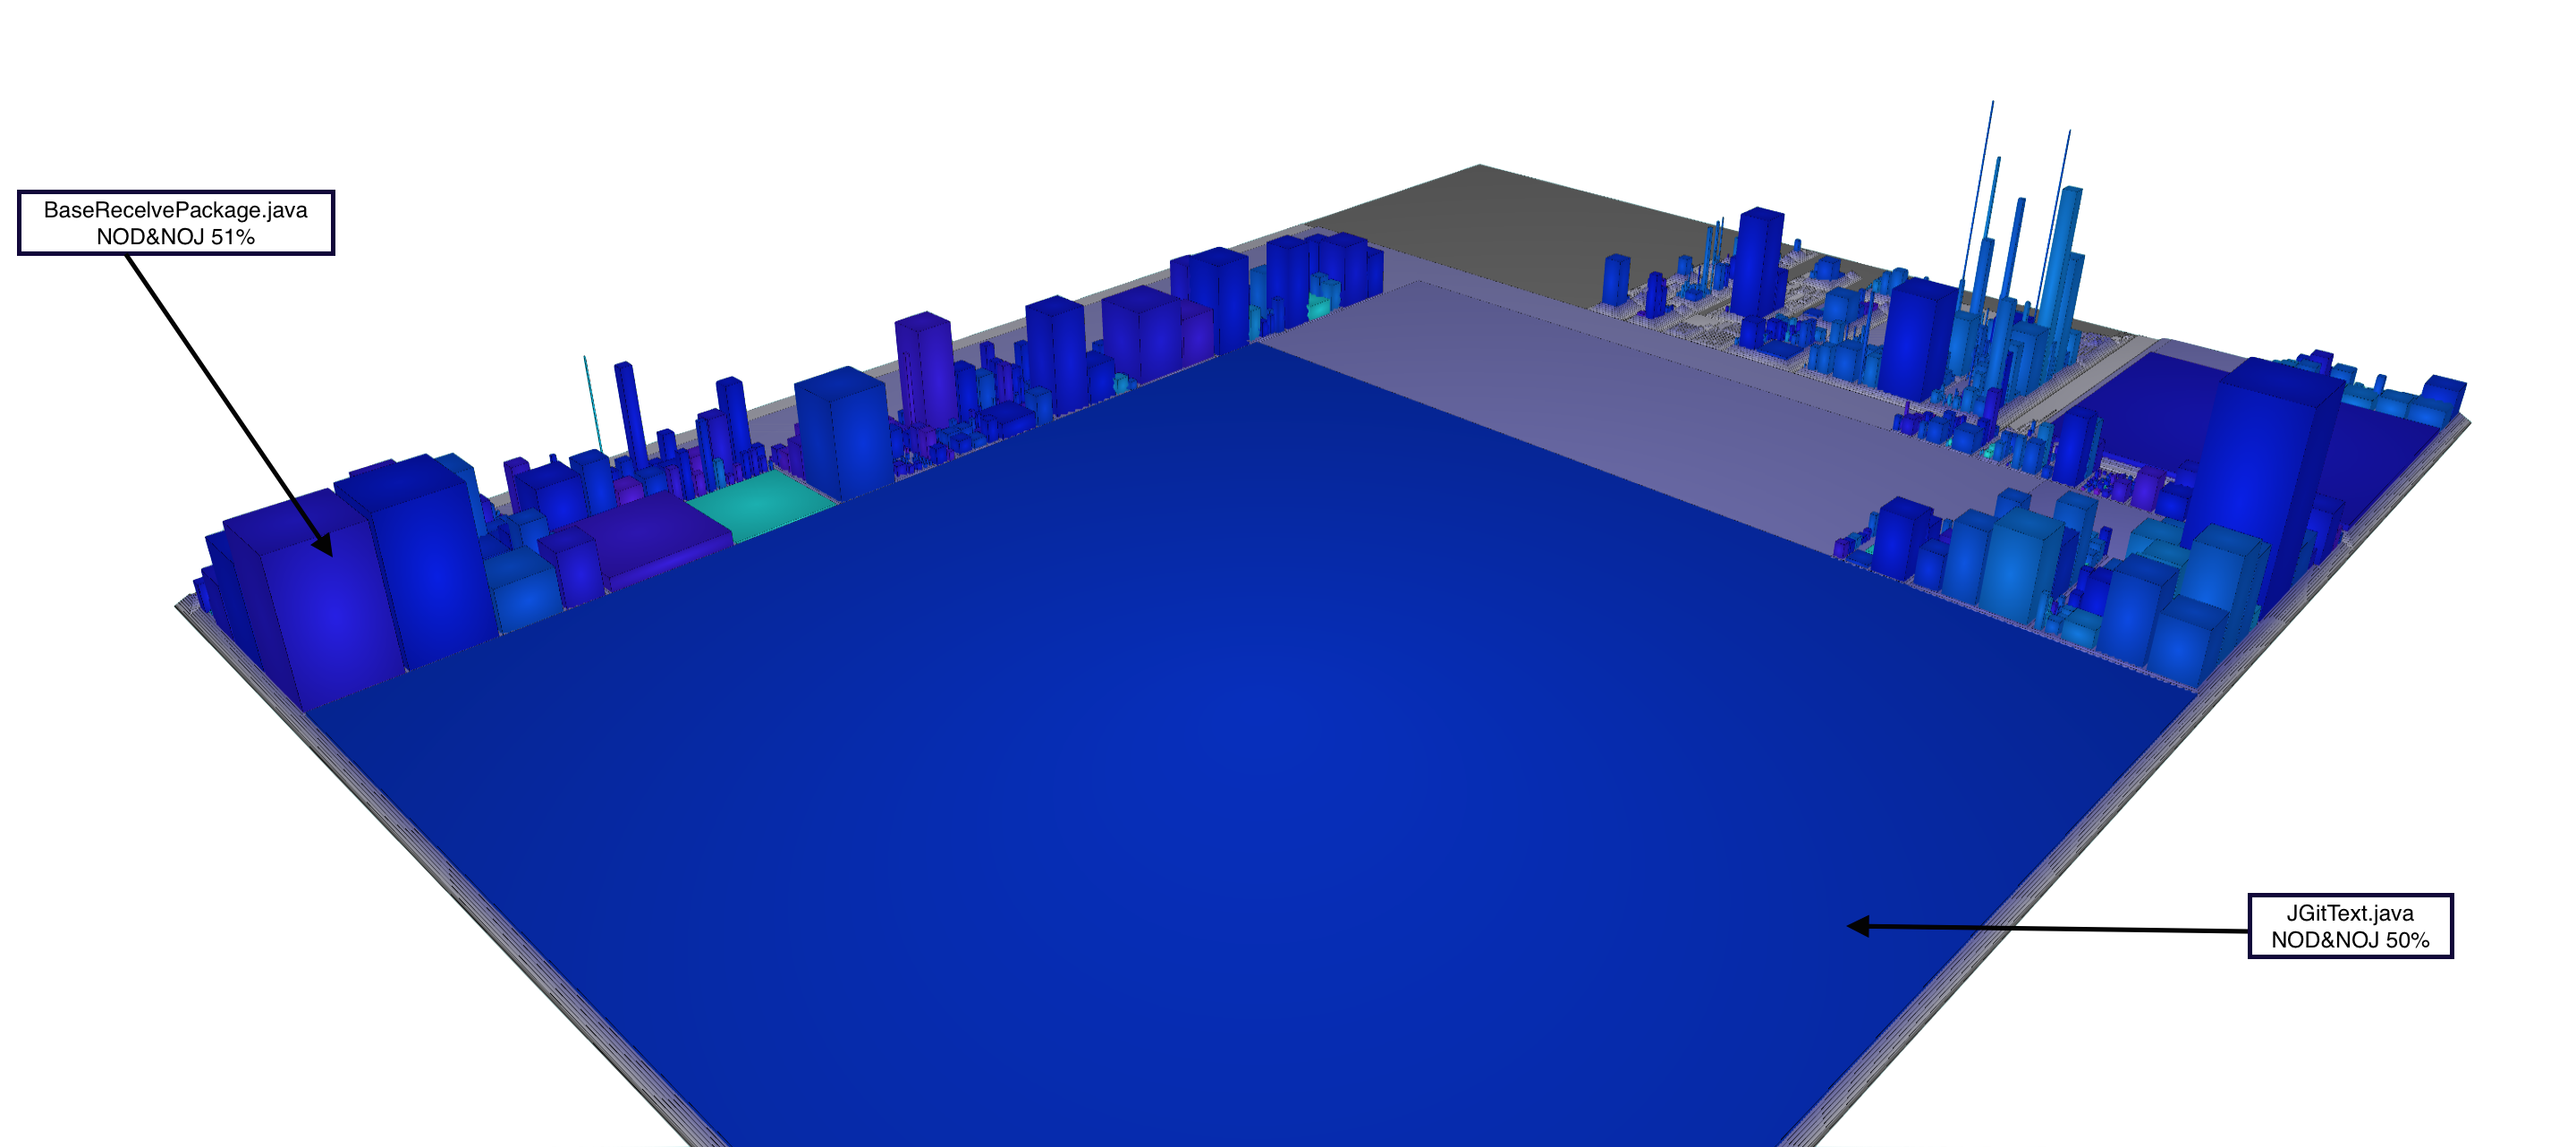
\includegraphics[width=0.95\textwidth]{images/jgitDocDisc}
	\caption[JGit: Discussion and Java Doc]{JGit: Discussion and Java Documentation express in percentage  \label{fig:jgitCorrollary:c}}
\end{figure}
Figure  \ref{fig:jgitCorrollary:c} shows a mix of both information. In general, we achieve a good level of information coverage of the entire system. There are two interesting points in this view: the former is  visually the more evident, the mix of JavaDoc and discussions on  \textit{JGitText.java} result in a bluish, this mean that we have around the 50\% of knowledge on it. The latter, the package \textit{jgit.interna.storage.file} that has not too much documentation, it has a lot  of discussions and therefore the information coverage is augmented. 














\newpage
\section{Conclusion} \label{conclusion}
We presented Cub8, a novel approach to extract information not strictly related to the code useful to improve the simplicity of understanding the system. It is the combination of an augmented visualization system using a 3d city metaphor with information that are retrieve from the web. We showed the possible information that it can visualize, it allows to analyze the information coverage as forum discussions or Java documentation individually, or it can combine multiple view to give to the developers a global idea about the system. Thanks to the possibility to change the metrics dynamically, we allow the developers to retrieve also some code disharmony. The user cases give to the developer an idea about how the system works and how is possible to highlight different problems of the system.
  
  

\newpage

\bibliographystyle{abbrv}
\bibliography{references}

\end{document}